%%%%%%%%%%%%%%%%%%%%%%%%%%%%%%%%%%%%%%%%%
% Short Sectioned Assignment LaTeX Template Version 1.0 (5/5/12)
% This template has been downloaded from: http://www.LaTeXTemplates.com
% Original author:  Frits Wenneker (http://www.howtotex.com)
% License: CC BY-NC-SA 3.0 (http://creativecommons.org/licenses/by-nc-sa/3.0/)
%%%%%%%%%%%%%%%%%%%%%%%%%%%%%%%%%%%%%%%%%

%----------------------------------------------------------------------------------------
%	PACKAGES AND OTHER DOCUMENT CONFIGURATIONS
%----------------------------------------------------------------------------------------

\documentclass[paper=a4, fontsize=11pt]{scrartcl} % A4 paper and 11pt font size

% ---- Entrada y salida de texto -----

\usepackage{hyperref}
\usepackage{varioref}
\usepackage[T1]{fontenc} % Use 8-bit encoding that has 256 glyphs
\usepackage[utf8]{inputenc}
%\usepackage{fourier} % Use the Adobe Utopia font for the document - comment this line to return to the LaTeX default

% ---- Idioma --------

\usepackage[spanish, es-tabla]{babel} % Selecciona el español para palabras introducidas automáticamente, p.ej. "septiembre" en la fecha y especifica que se use la palabra Tabla en vez de Cuadro

% ---- Otros paquetes ----

\usepackage{amsmath,amsfonts,amsthm} % Math packages
%\usepackage{graphics,graphicx, floatrow} %para incluir imágenes y notas en las imágenes
\usepackage{graphics,graphicx, float} %para incluir imágenes y colocarlas

% Para hacer tablas comlejas
%\usepackage{multirow}
%\usepackage{threeparttable}

%\usepackage{sectsty} % Allows customizing section commands
%\allsectionsfont{\centering \normalfont\scshape} % Make all sections centered, the default font and small caps

\usepackage{fancyhdr} % Custom headers and footers
\pagestyle{fancyplain} % Makes all pages in the document conform to the custom headers and footers
\fancyhead{} % No page header - if you want one, create it in the same way as the footers below
\fancyfoot[L]{} % Empty left footer
\fancyfoot[C]{} % Empty center footer
\fancyfoot[R]{\thepage} % Page numbering for right footer
\renewcommand{\headrulewidth}{0pt} % Remove header underlines
\renewcommand{\footrulewidth}{0pt} % Remove footer underlines
\setlength{\headheight}{13.6pt} % Customize the height of the header

\numberwithin{equation}{section} % Number equations within sections (i.e. 1.1, 1.2, 2.1, 2.2 instead of 1, 2, 3, 4)
\numberwithin{figure}{section} % Number figures within sections (i.e. 1.1, 1.2, 2.1, 2.2 instead of 1, 2, 3, 4)
\numberwithin{table}{section} % Number tables within sections (i.e. 1.1, 1.2, 2.1, 2.2 instead of 1, 2, 3, 4)

\setlength\parindent{0pt} % Removes all indentation from paragraphs - comment this line for an assignment with lots of text

\newcommand{\horrule}[1]{\rule{\linewidth}{#1}} % Create horizontal rule command with 1 argument of height


%----------------------------------------------------------------------------------------
%	TÍTULO Y DATOS DEL ALUMNO
%----------------------------------------------------------------------------------------

\title{	
\normalfont \normalsize 
\textsc{{\bf Ingeniería de Servidores (2015-2016)} \\ Grado en Ingeniería Informática \\ Universidad de Granada} \\ [25pt] % Your university, school and/or department name(s)
\horrule{0.5pt} \\[0.4cm] % Thin top horizontal rule
\huge Memoria Práctica 4 \\ % The assignment title
\horrule{2pt} \\[0.5cm] % Thick bottom horizontal rule
}

\author{Francisco Carrillo Pérez} % Nombre y apellidos

\date{\normalsize\today} % Incluye la fecha actual

%----------------------------------------------------------------------------------------
% DOCUMENTO
%----------------------------------------------------------------------------------------

\begin{document}

\maketitle % Muestra el Título

\newpage %inserta un salto de página

\tableofcontents % para generar el índice de contenidos

\listoffigures

\listoftables

\newpage

%%%%%%%%%%%%%%%%%%%%%%%%%%%%%%%%%%%%%%%%%%%%%%%%%%%%
% CUESTIÓN 1
%%%%%%%%%%%%%%%%%%%%%%%%%%%%%%%%%%%%%%%%%%%%%%%%%%%%

\section{Cuestión 1: Instale la aplicación. ¿Qué comando permite listar los benchmarks disponibles?}

Para instalar la suite podemos hacer uso del siguiente comando en Ubuntu \cite{phoronix-suite}:\\
\textbf{sudo apt-get install phoronix-test-suite}\\

Para ver la lista de benchmarks disponible podemos usar el siguiente comando \cite{phoronix-suite}:\\
\textbf{phoronix-test-suite list-available-tests}

\begin{figure}[H] %con el [H] le obligamos a situar aquí la figura
	\centering
	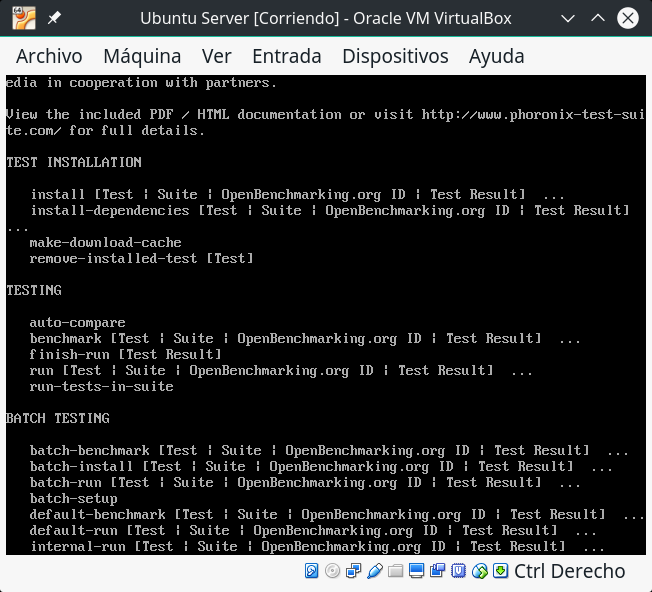
\includegraphics[scale=0.5]{figuras/figura1.png}  %el parámetro scale permite agrandar o achicar la imagen. En el nombre de archivo puede especificar directorios
	\label{figura1}
	
	\caption{Resultado al ejecutar \textbf{phoronix-test-suite list-available-tests}}
\end{figure}

\begin{figure}[H] %con el [H] le obligamos a situar aquí la figura
	\centering
	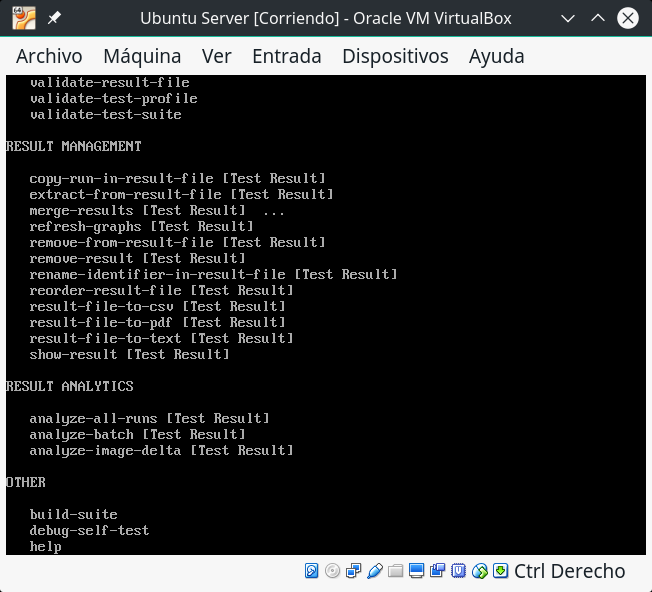
\includegraphics[scale=0.5]{figuras/figura2.png}  %el parámetro scale permite agrandar o achicar la imagen. En el nombre de archivo puede especificar directorios
	\label{figura2}
	
	\caption{Resultado al ejecutar \textbf{phoronix-test-suite list-available-tests}}
\end{figure}

%%%%%%%%%%%%%%%%%%%%%%%%%%%%%%%%%%%%%%%%%%%%%%%%%%%%
% CUESTIÓN 2
%%%%%%%%%%%%%%%%%%%%%%%%%%%%%%%%%%%%%%%%%%%%%%%%%%%%

\section{Cuestión 2:}

\subsection{De los parámetros que le podemos pasar al comando ¿Qué significa -c 5 ?}
Gracias  a la página del man del comando ab \cite{ab} podemos saber que la opción -c 5 indica que queremos que se envién 5 peticiones cada vez.
\subsection{¿y -n 100?}
Gracias  a la página del man del comando ab \cite{ab} podemos saber que la opción -n 100 lo que indica es que se envíen 100 peticiones durante la ejecución del benchmark.
\subsection{Monitorice la ejecución de ab contra alguna máquina (cualquiera) ¿cuántos procesos o hebras crea ab en el cliente?}

Para ejecutarlo debemos hacer uso del siguiente comando: \textbf{ab -n 10000 -c 50 http://192.168.56.2/}\\
La barra es muy importante ya que nos coge el path por defecto que es el index.html.

El resultado de la ejecucion es el que podemos observar en la Figura \ref{figura4}\\
Con el comando \textbf{ps -Af |  grep ab | wc -l} contabilizamos cuántos procesos ab hay en la máquina cliente y con el comando \textbf{ps -Af |  grep apache2 | wc -l} contabilizamos las procesos de apache2 en el servidor.
En el cliente ab sólo crea una hebra de ab (se muestran 2 porque cuenta la línea del grep). En cambio en el servidor que es contra el cuál ejecutamos ab podemos observar que se crean casi tantos servicios de apache2 como peticiones concurrentes hemos indicado con -c. No se crean todas porque va ejecutando por ráfagas entonces no podemos contabilizarlas directamente.

\begin{figure}[H] %con el [H] le obligamos a situar aquí la figura
	\centering
	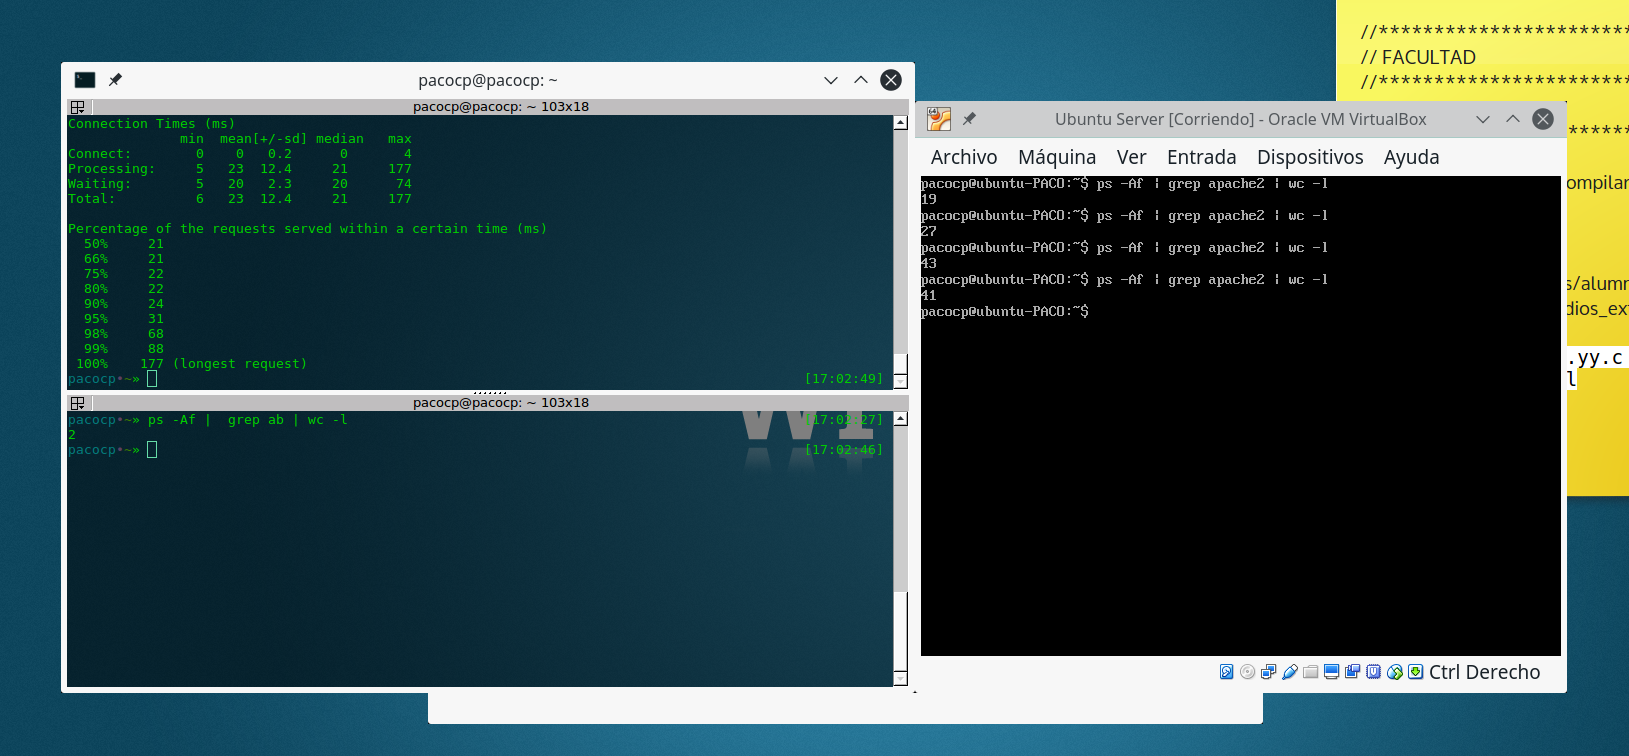
\includegraphics[scale=0.35]{figuras/figura4.png}  %el parámetro scale permite agrandar o achicar la imagen. En el nombre de archivo puede especificar directorios
	
	
	\caption{Resultado al ejecutar \textbf{ab -n 10000 -c 50 http://192.168.56.2/}}
	\label{figura4}
\end{figure}

%%%%%%%%%%%%%%%%%%%%%%%%%%%%%%%%%%%%%%%%%%%%%%%%%%%%
% CUESTIÓN 3
%%%%%%%%%%%%%%%%%%%%%%%%%%%%%%%%%%%%%%%%%%%%%%%%%%%%

\section{Cuestión 3: Ejecute ab contra a las tres máquinas virtuales (desde el SO anfitrión a las máquina virtuales de la red local) una a una (arrancadas por separado) y muestre y comente las estadísticas. ¿Cuál es la que proporciona mejores resultados? Fíjese en el número de bytes transferidos, ¿es igual para cada máquina?}

Vamos a realizar la ejecución del comando ab contra las tres máquinas de la siguiente forma: \textbf{ab -n 10000 -c 50} .\\
Podemos observar los resultados en las siguientes imágenes.
\begin{itemize}
	\item En la Figura \ref{figura5} podemos observar la ejecución contra la máquina con Ubuntu Server. Podemos observar que ha tardado 5.100 segundos. En este caso el número de bytes transferidos es de 117830000 bytes.
	\item En la Figura \ref{figura6} podemos observar la ejecución contra la máquina con CentOS. Podemos observar que ha tardado 6.358 segundos. En este caso el número de bytes transferidos es de 51680000 bytes.
	\item Por último, en la Figura \ref{figura7} podemos observar la ejecución contra la máquina con CentOS. Podemos observar que ha tardado 3.721 segundos. En este caso el número de bytes transferidos es de 9310000 bytes.
\end{itemize} 

Si observamos las estadísticas de todos los benchmark podemos observar que en todos se realizan las mismas peticiones, ya que son las que le hemos indicado con el comando. También podemos observar el tiempo por petición, en el caso de \textbf{Ubuntu Server \ref{figura5}} el valor es de 25,502 ms, en el caso de \textbf{CentOS \ref{figura6}} el valor es de 31,792 ms y por último en el caso de \textbf{Windows Server \ref{figura7}} el valor es de 18,607 ms.\\
Podemos observar en la Figura  \ref{figura8} que la máquina más rápida es aquella con Windows Server seguida de la de Ubuntu Server. Esto se debe a que Windows tiene activada por defecto la opción de compresión de http y gzip \cite{gzip} \cite{http-comp}.Esto también se puede observar en el tiempo por petición que hemos observado en el párrafo superior, siendo el de Windows Server el más rápido.\\
En cambio, podemos observar en la Figura \ref{figura9} que la máquina que más bytes transfiere es aquella con Ubuntu Server. Esto se debe a o mismo anteriormente nombrado, y es que los datos que envía Windows Server vienen por defecto comprimidos.

\begin{figure}[H] %con el [H] le obligamos a situar aquí la figura
	\centering
	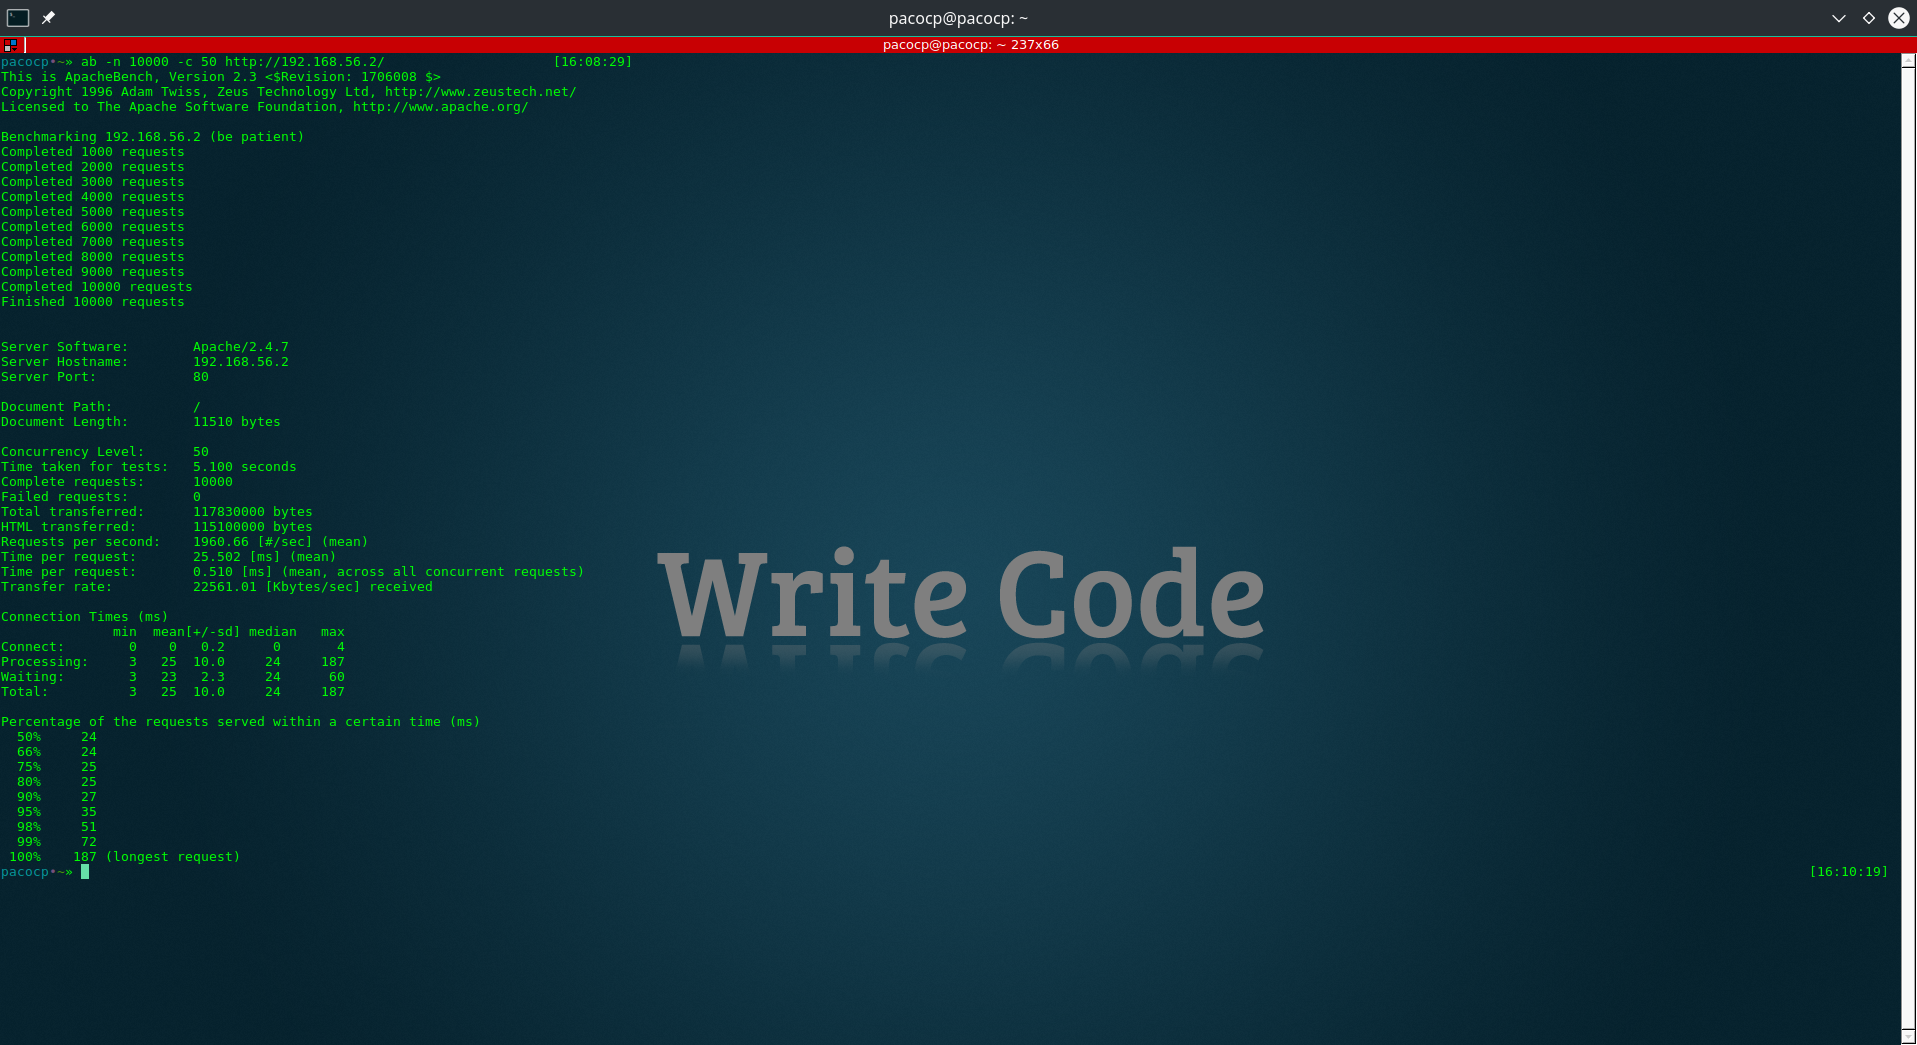
\includegraphics[scale=0.35]{figuras/figura5.png}  %el parámetro scale permite agrandar o achicar la imagen. En el nombre de archivo puede especificar directorios
	
	
	\caption{Resultado al ejecutar \textbf{ab -n 10000 -c 50 http://192.168.56.2/}}
	\label{figura5}
\end{figure}

\begin{figure}[H] %con el [H] le obligamos a situar aquí la figura
	\centering
	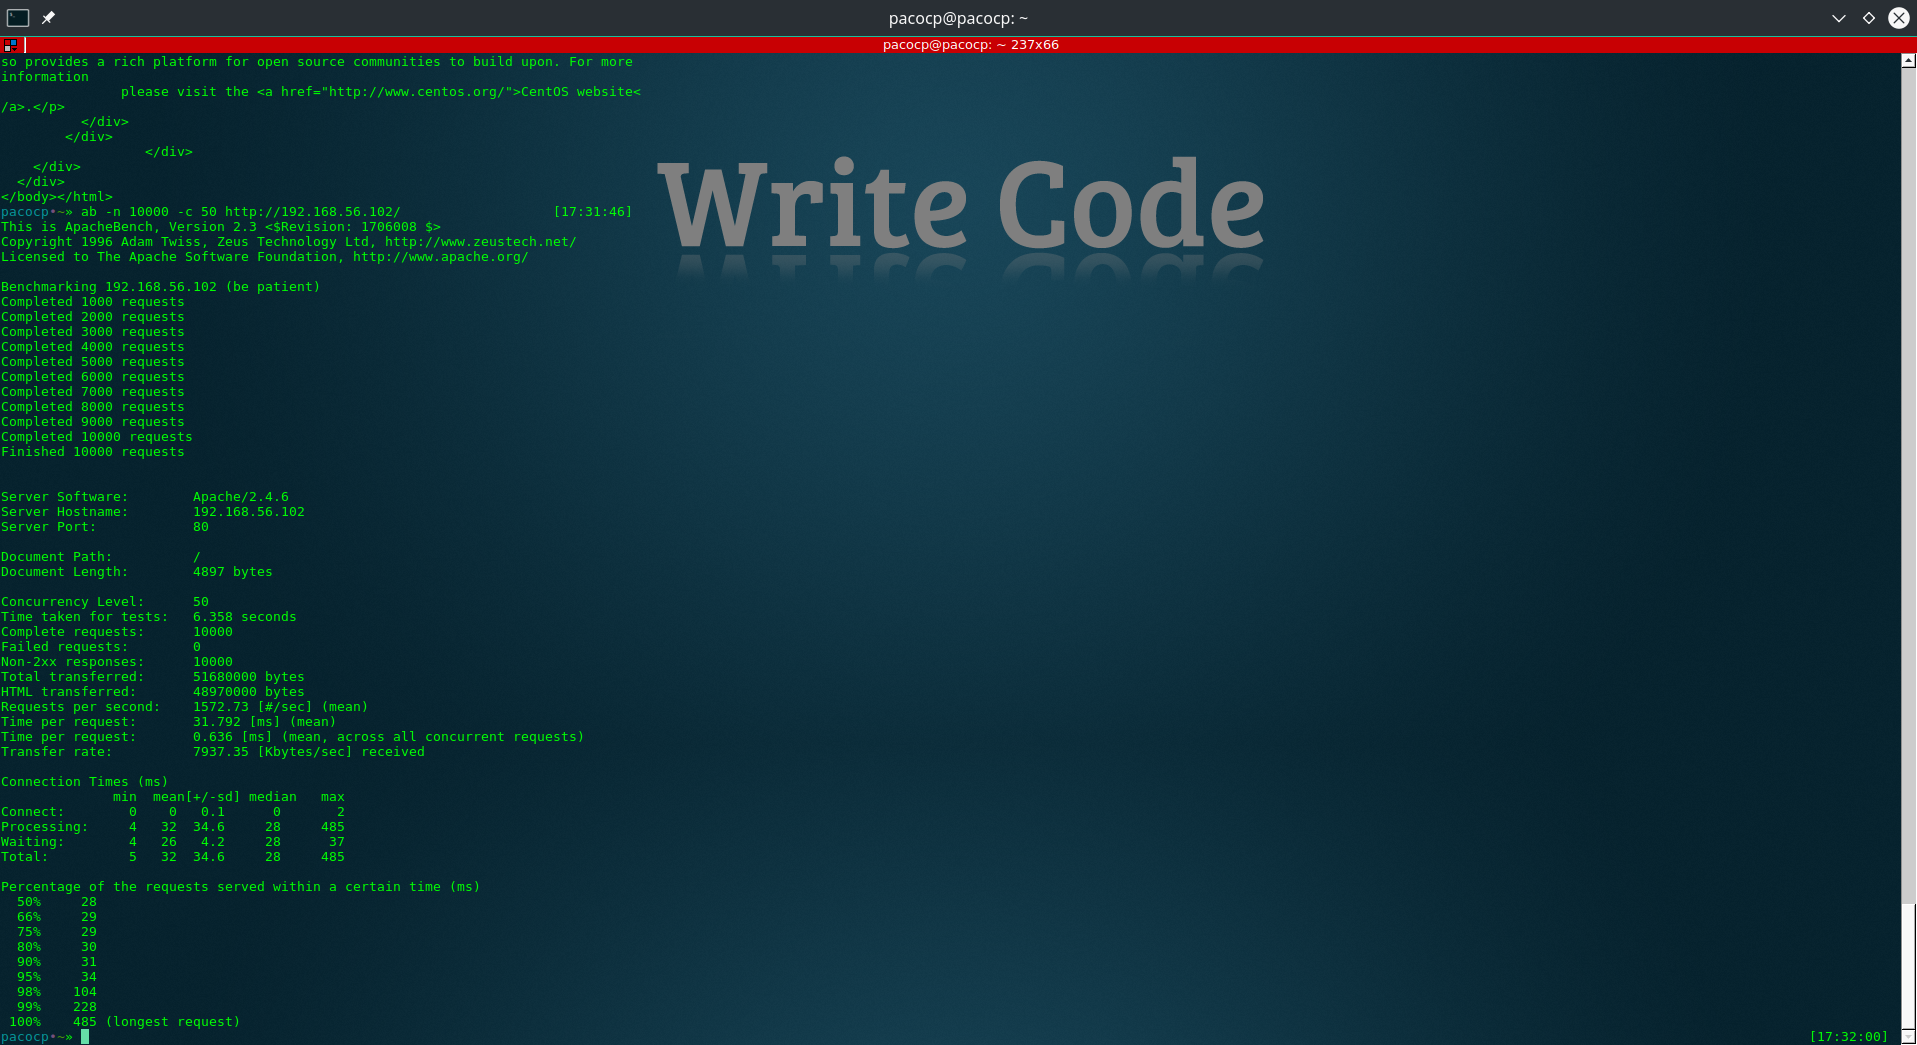
\includegraphics[scale=0.35]{figuras/figura6.png}  %el parámetro scale permite agrandar o achicar la imagen. En el nombre de archivo puede especificar directorios
	
	
	\caption{Resultado al ejecutar \textbf{ab -n 10000 -c 50 http://192.168.56.102/}}
	\label{figura6}
\end{figure}
\begin{figure}[H] %con el [H] le obligamos a situar aquí la figura
	\centering
	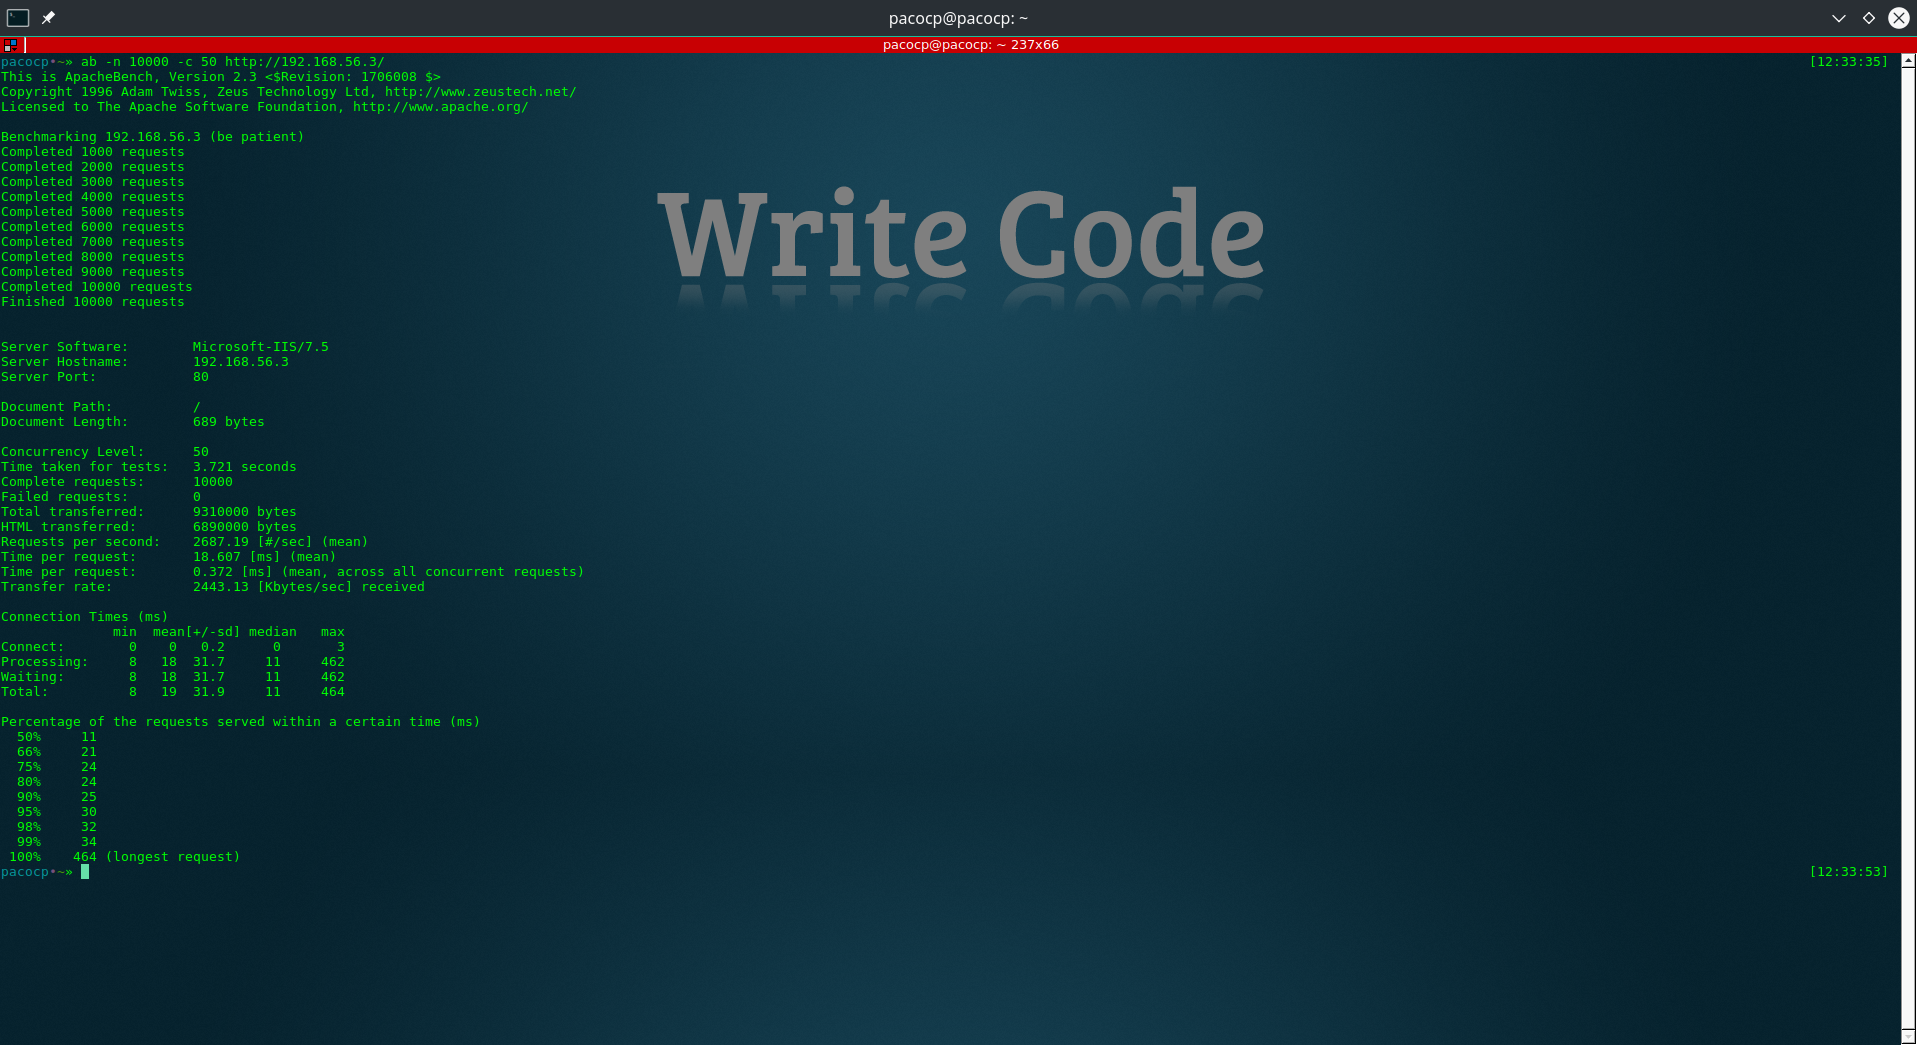
\includegraphics[scale=0.35]{figuras/figura7.png}  %el parámetro scale permite agrandar o achicar la imagen. En el nombre de archivo puede especificar directorios
	
	
	\caption{Resultado al ejecutar \textbf{ab -n 10000 -c 50 http://192.168.56.3/}}
	\label{figura7}
\end{figure}

\begin{figure}[H] %con el [H] le obligamos a situar aquí la figura
	\centering
	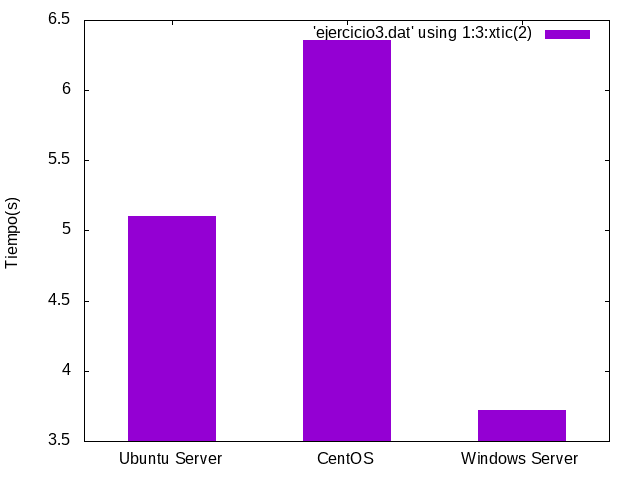
\includegraphics[scale=0.5]{figuras/figura8.png}  %el parámetro scale permite agrandar o achicar la imagen. En el nombre de archivo puede especificar directorios
	
	
	\caption{Tiempo de ejecución (s)}
	\label{figura8}
\end{figure}
\begin{figure}[H] %con el [H] le obligamos a situar aquí la figura
	\centering
	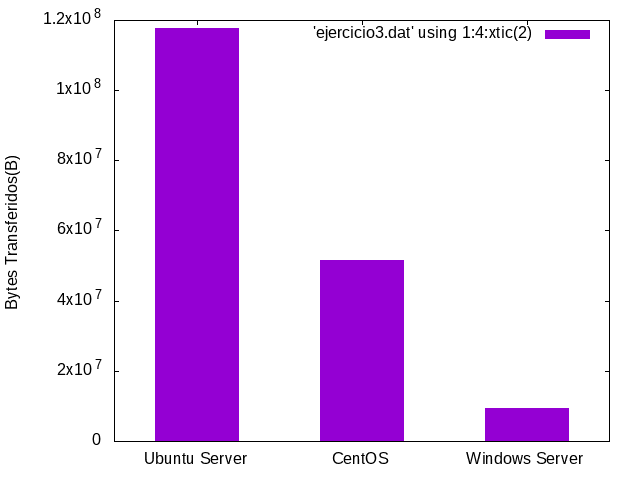
\includegraphics[scale=0.5]{figuras/figura9.png}  %el parámetro scale permite agrandar o achicar la imagen. En el nombre de archivo puede especificar directorios
	
	
	\caption{Bytes transferidos}
	\label{figura9}
\end{figure}
%%%%%%%%%%%%%%%%%%%%%%%%%%%%%%%%%%%%%%%%%%%%%%%%%%%%
% CUESTIÓN 4
%%%%%%%%%%%%%%%%%%%%%%%%%%%%%%%%%%%%%%%%%%%%%%%%%%%%

\section{Cuestión 4: Instale y siga el tutorial en http://jmeter.apache.org/usermanual/build-web-test-plan.html realizando capturas de pantalla y comentándolas. En vez de usar la web de jmeter, haga el experimento usando alguna de sus máquinas virtuales (Puede hacer una página sencilla, usar las páginas de phpmyadmin, instalar un CMS, etc.).}

En mi caso voy a instalar jmeter en una máquina con Manjaro como sistema operativo. Para poder instalajar jmeter es necesario añadir su clave pública para verificar los paquetes para ello es necesario descargarse el archivo con las KEYS de la página \cite{keys}. Para instalarlas usamos el siguiente comando \textbf{gpg --import KEYS},en la Figura \ref{figura12} podemos observar el resultado.\\
Ahora ya podemos instalarlo haciendo uso del comando \textbf{yaourt -S jmeter} .\\

\begin{figure}[H] %con el [H] le obligamos a situar aquí la figura
	\centering
	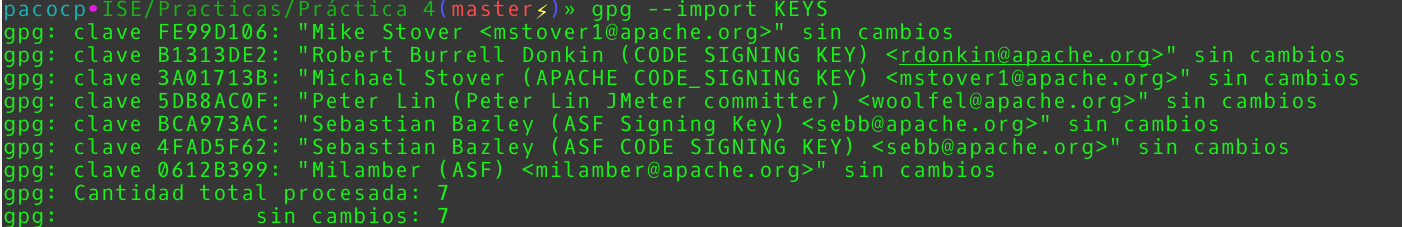
\includegraphics[scale=0.35]{figuras/figura12.png}  %el parámetro scale permite agrandar o achicar la imagen. En el nombre de archivo puede especificar directorios
	
	
	\caption{Importando las KEYS \textbf{gpg --import KEYS}}
	\label{figura12}
\end{figure}

Si abrimos jmeter podemos observar lo que nos muestra de inicio en la Figura \ref{figura13}. Ahora vamos a realizar el tutorial.\\

\begin{enumerate}
	\item Añadimos un grupo de hilos,Figura \ref{figura14}.Le ponemos de nombre JMeter Users, aumentamos el número de hilos a 2 y el contador del bucle lo ponemos a 2000. Podemos observar como quedaría en la Figura \ref{figura15}.
	\item Ahora vamos a definir las tareas que van a realizar los usuarios, especificando los apuntes de las peticiones HTTP. Pulsando sobre el grupo de hilos que hemos creado le damos a añadir->elemento de configuración->valores por defecto para petición HTTP.  Se nos mostrará de la forma que podemos observar en la Figura \ref{figura16}. Ahora lo único que vamos a definir es al servidor al que vamos a hacer las peticiones. En este caso vamos a utilizar la página web simple creada en la máquina con CentOS, \textbf{http://192.168.56.102/index.html/}, podemos ver el código en la Figura \ref{figura23}. Podemos observarlo en la Figura \ref{figura17}. 
	\item Vamos a añadir el soporte para las cookies. Se añaden con el botón derecho sobre el grupo de hilos añadir->elemento de configuración->gestor de cookies HTTP. Podemos observar como quedaría en la Figura \ref{figura18}.
	\item Ahora vamos a añadir una petición HTTP al raíz de la página que he creado. Para ello sobre el grupo de threads pulsamos  añadir->muestreador->petición HTTP. Le cambiamos el nombre a Home Page y ponemos en la ruta raíz. Quedaría como podemos ver en la Figura \ref{figura19} . 
	\item Por último, tenemos que añadir un Receptor. Para ello pulsamos botón derecho y añadir->receptor->gráfico de resultados. Y configuramos donde queremos guardarlo, como podemos observar en la Figura \ref{figura20}
\end{enumerate}

Si ejecutamos, podremos ver los resultados en tiempo real en la pestaña  gráfico de resultados, que podemos ver en la Figura \ref{figura24}. En ella vemos como al final la media y la mediana se acercan a 1 ms.
\begin{figure}[H] %con el [H] le obligamos a situar aquí la figura
	\centering
	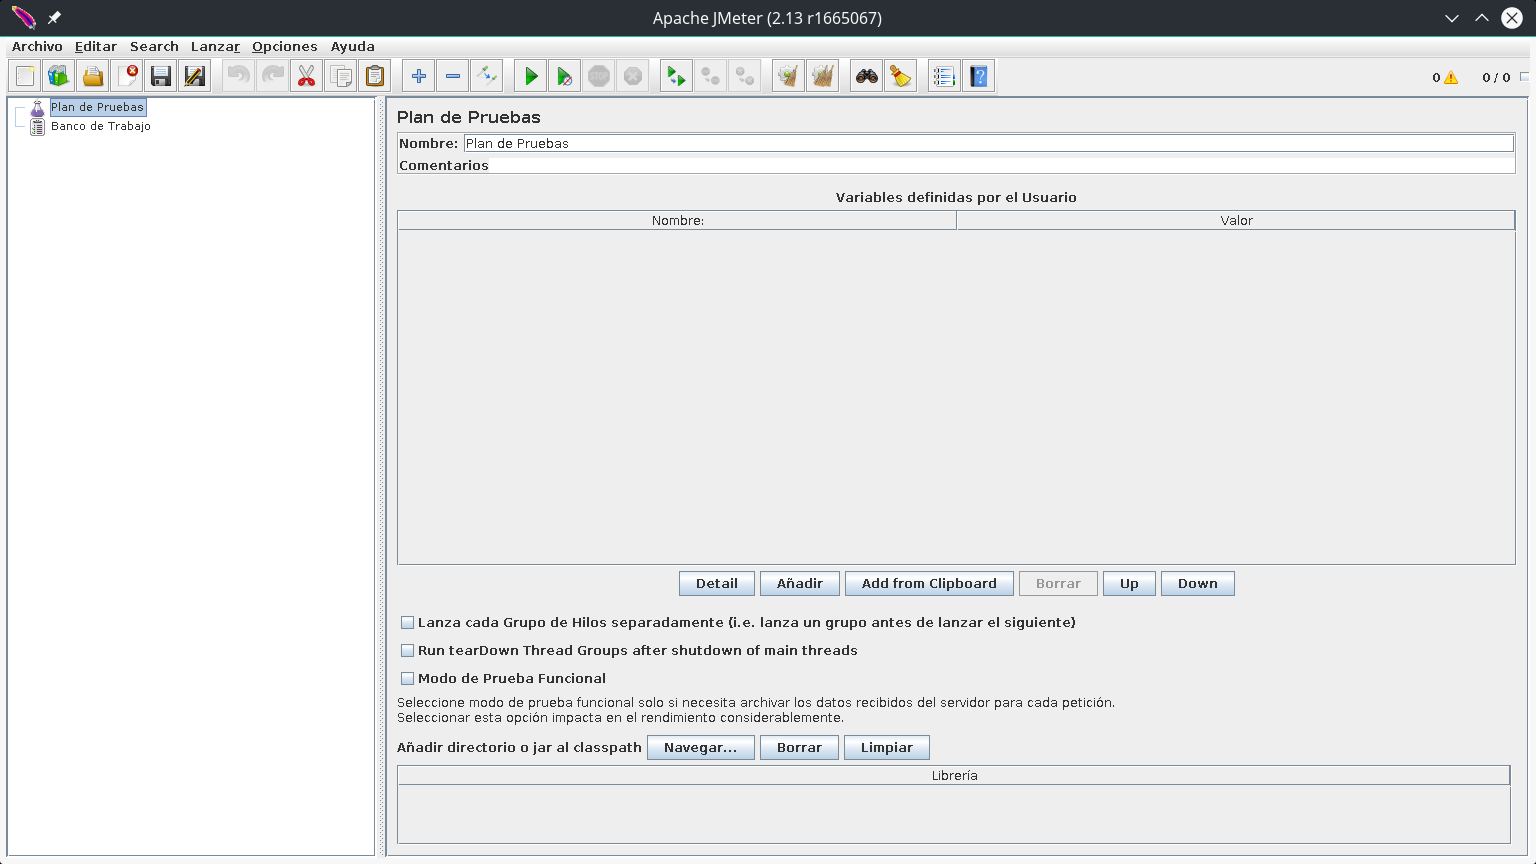
\includegraphics[scale=0.35]{figuras/figura13.png}  %el parámetro scale permite agrandar o achicar la imagen. En el nombre de archivo puede especificar directorios
	
	
	\caption{Página de inicio de jmeter}
	\label{figura13}
\end{figure}

\begin{figure}[H] %con el [H] le obligamos a situar aquí la figura
	\centering
	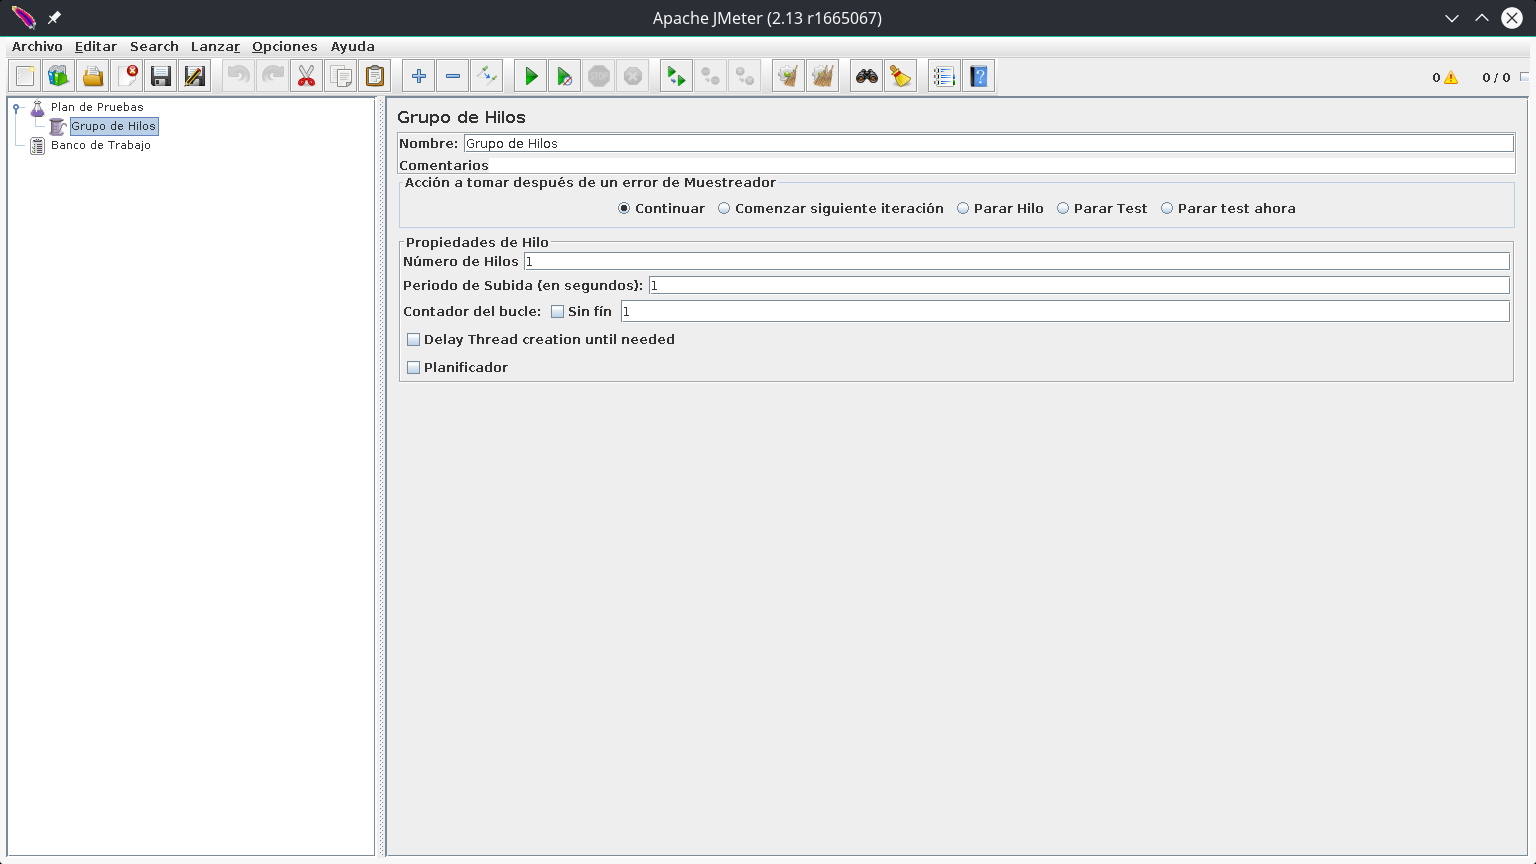
\includegraphics[scale=0.35]{figuras/figura14.png}  %el parámetro scale permite agrandar o achicar la imagen. En el nombre de archivo puede especificar directorios
	
	
	\caption{Grupo de hilos}
	\label{figura14}
\end{figure}

\begin{figure}[H] %con el [H] le obligamos a situar aquí la figura
	\centering
	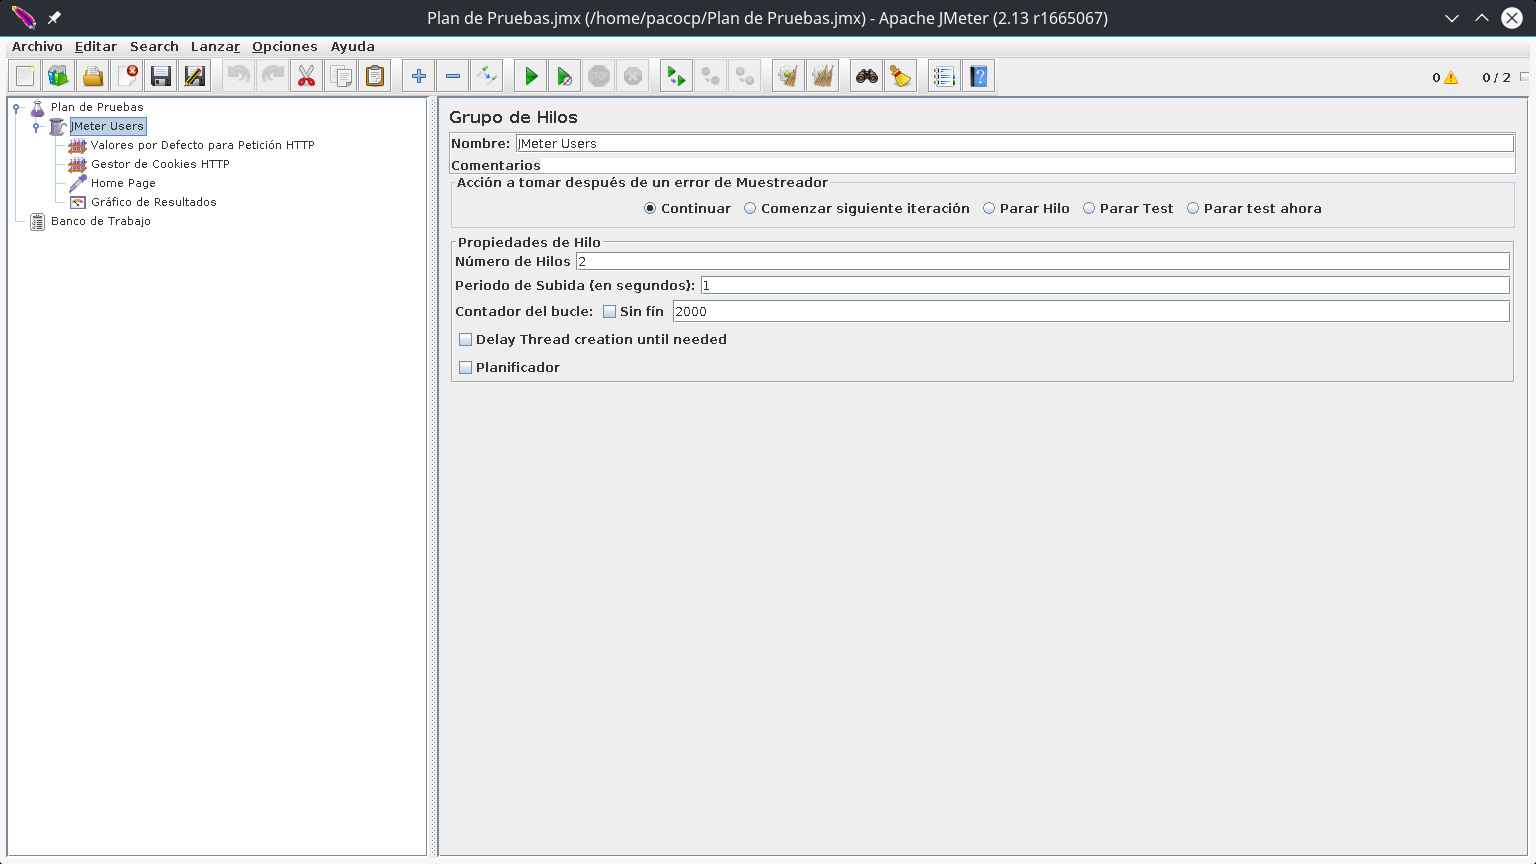
\includegraphics[scale=0.35]{figuras/figura15.png}  %el parámetro scale permite agrandar o achicar la imagen. En el nombre de archivo puede especificar directorios
	
	
	\caption{Grupo de hilos modificado}
	\label{figura15}
\end{figure}

\begin{figure}[H] %con el [H] le obligamos a situar aquí la figura
	\centering
	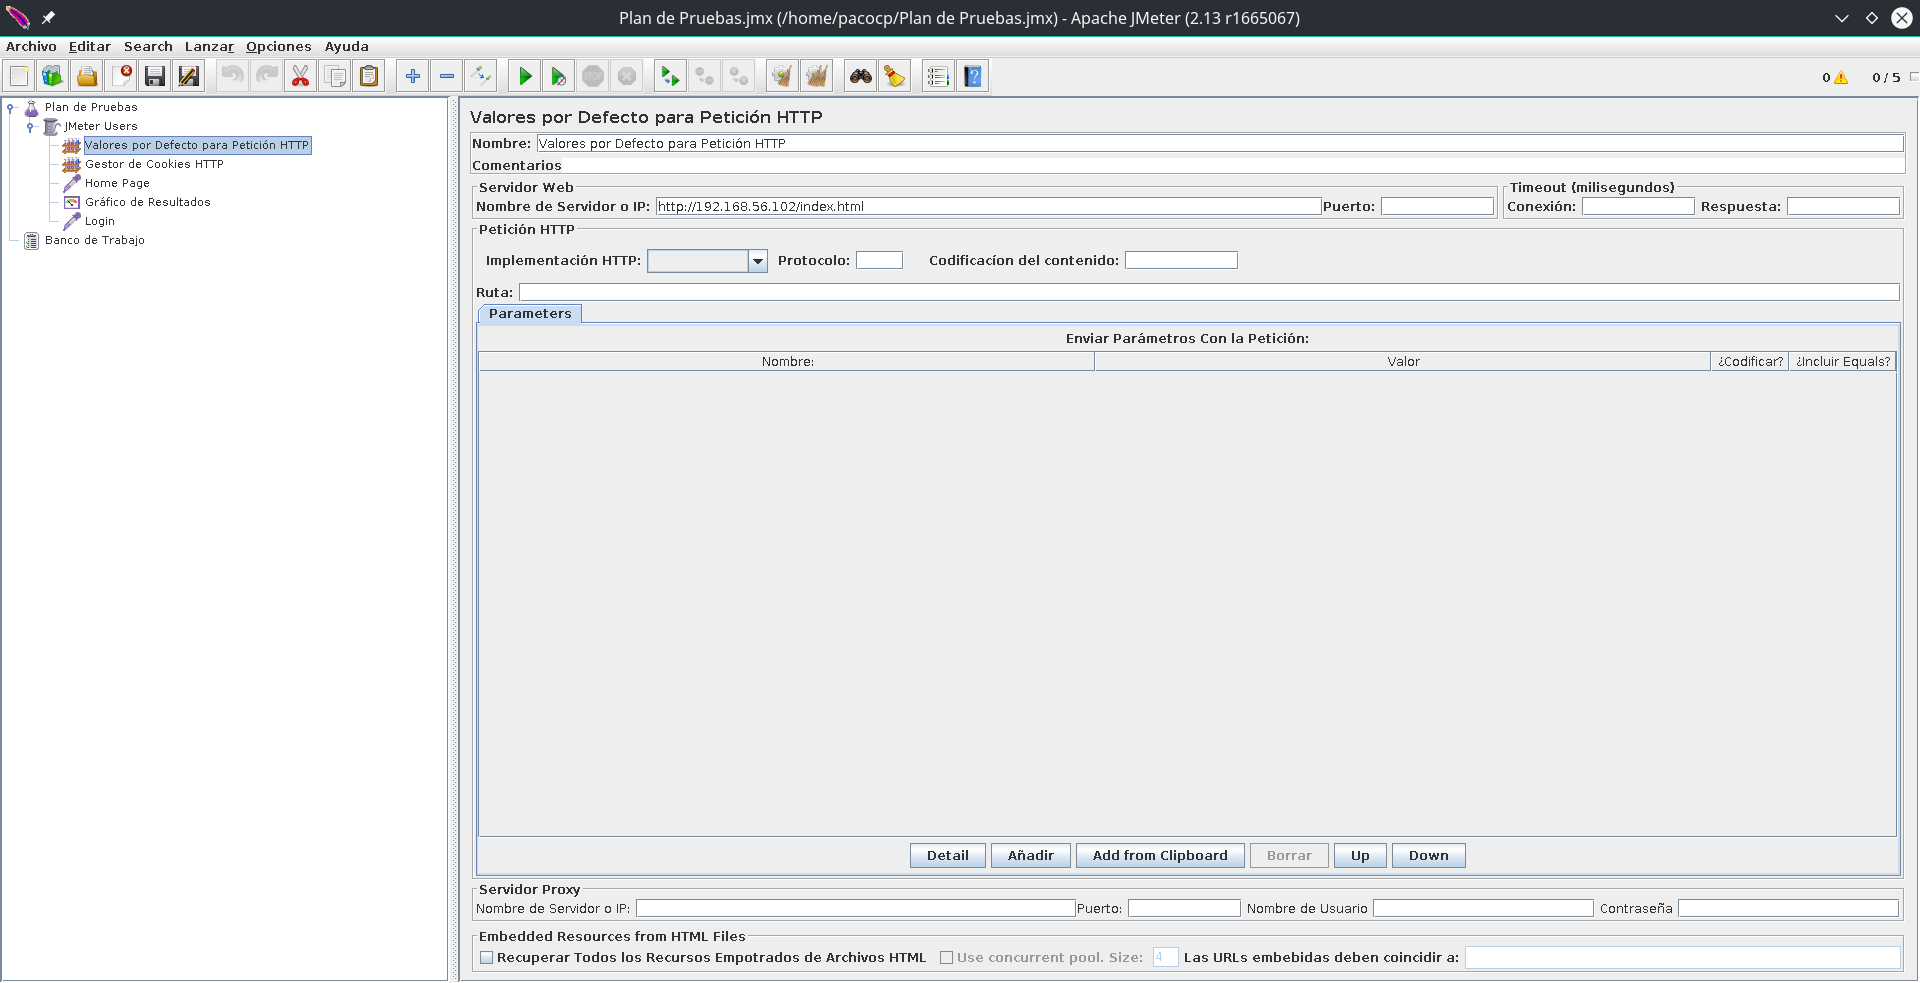
\includegraphics[scale=0.35]{figuras/figura16.png}  %el parámetro scale permite agrandar o achicar la imagen. En el nombre de archivo puede especificar directorios
	
	
	\caption{Valores por defecto para petición HTTP}
	\label{figura16}
\end{figure}

\begin{figure}[H] %con el [H] le obligamos a situar aquí la figura
	\centering
	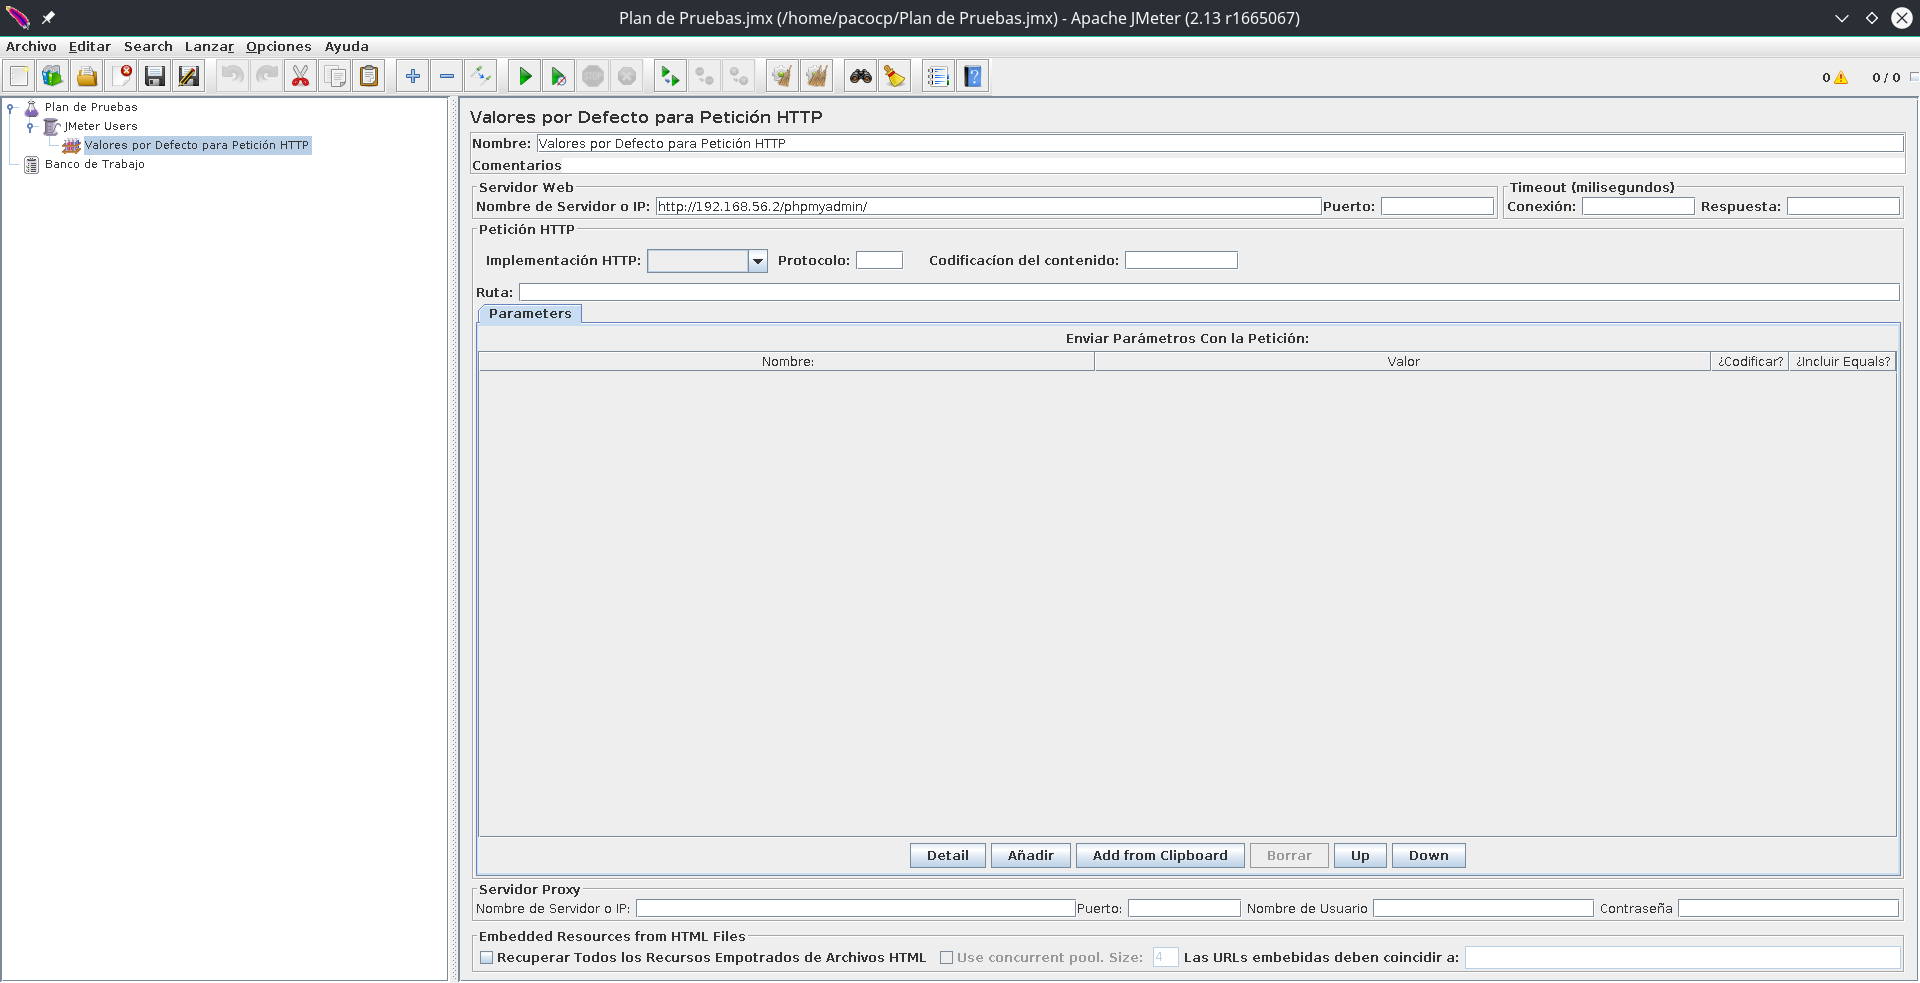
\includegraphics[scale=0.35]{figuras/figura17.png}  %el parámetro scale permite agrandar o achicar la imagen. En el nombre de archivo puede especificar directorios
	
	
	\caption{Configurada la página a la que se van a realizar las peticiones HTTP}
	\label{figura17}
\end{figure}

\begin{figure}[H] %con el [H] le obligamos a situar aquí la figura
	\centering
	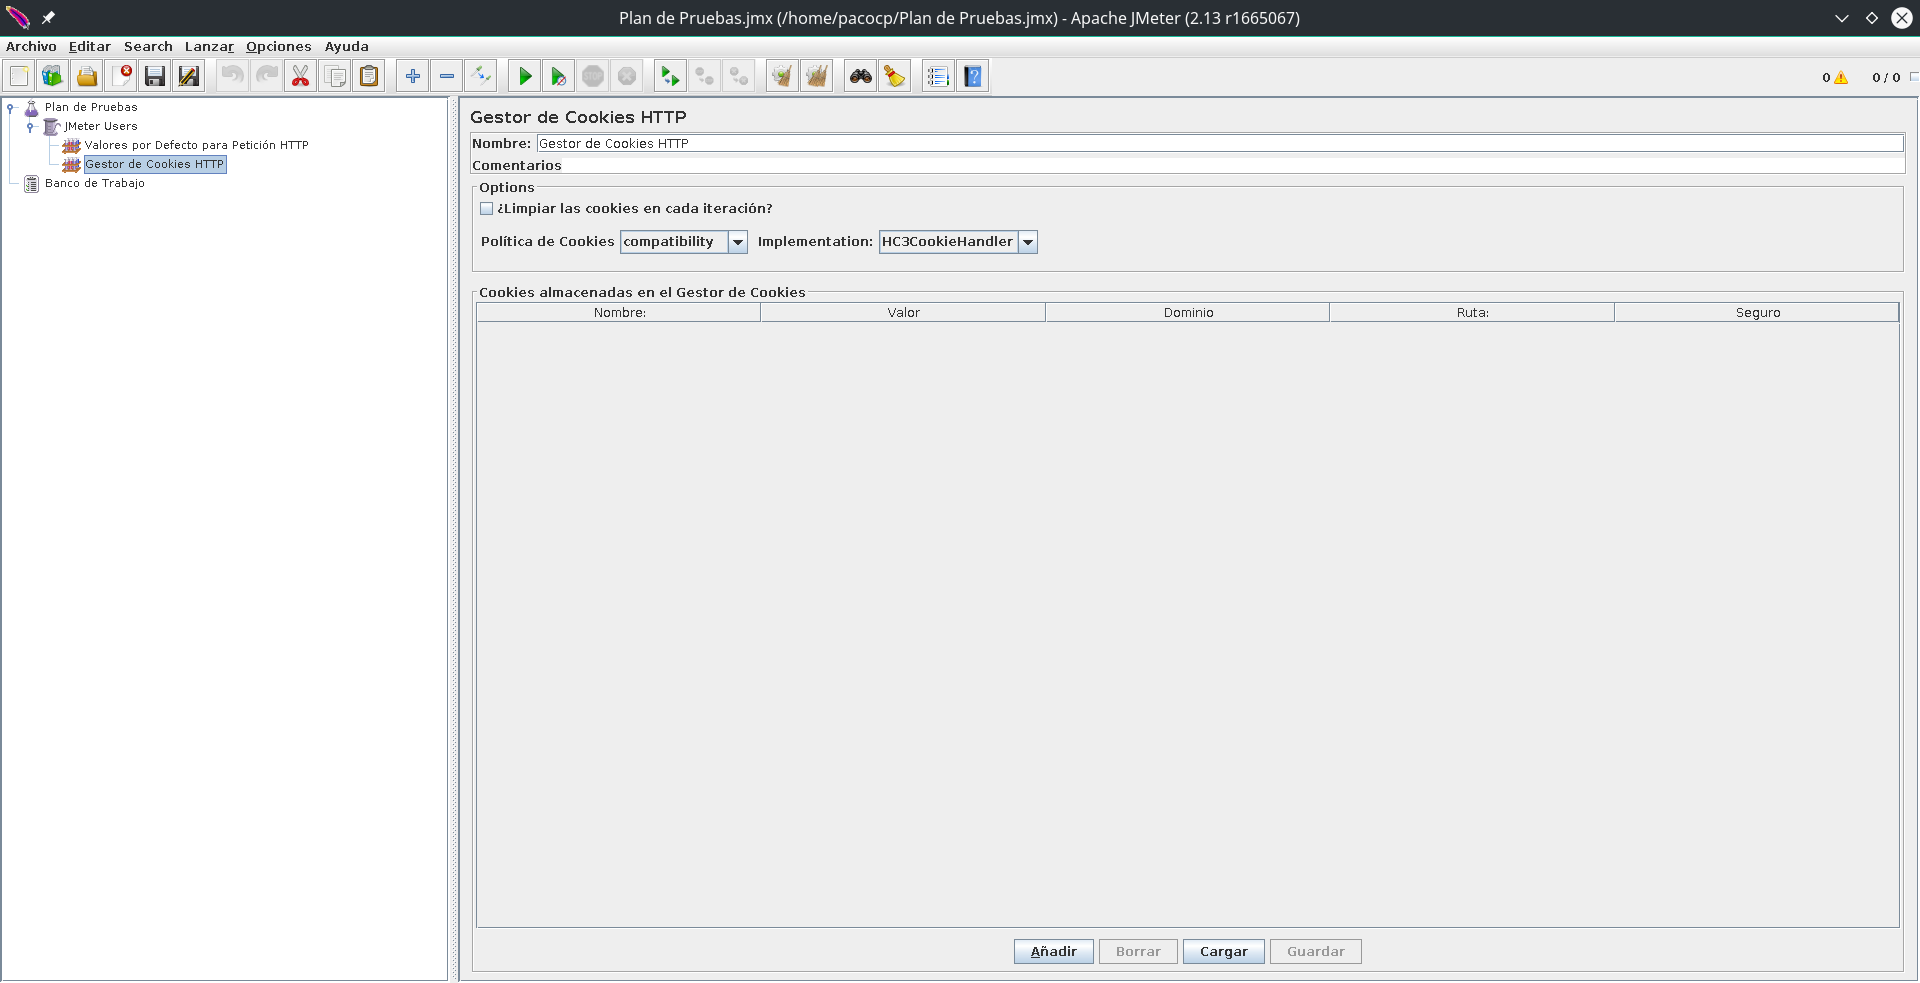
\includegraphics[scale=0.35]{figuras/figura18.png}  %el parámetro scale permite agrandar o achicar la imagen. En el nombre de archivo puede especificar directorios
	
	
	\caption{Configurado el Gesto de Cookies HTTP}
	\label{figura18}
\end{figure}

\begin{figure}[H] %con el [H] le obligamos a situar aquí la figura
	\centering
	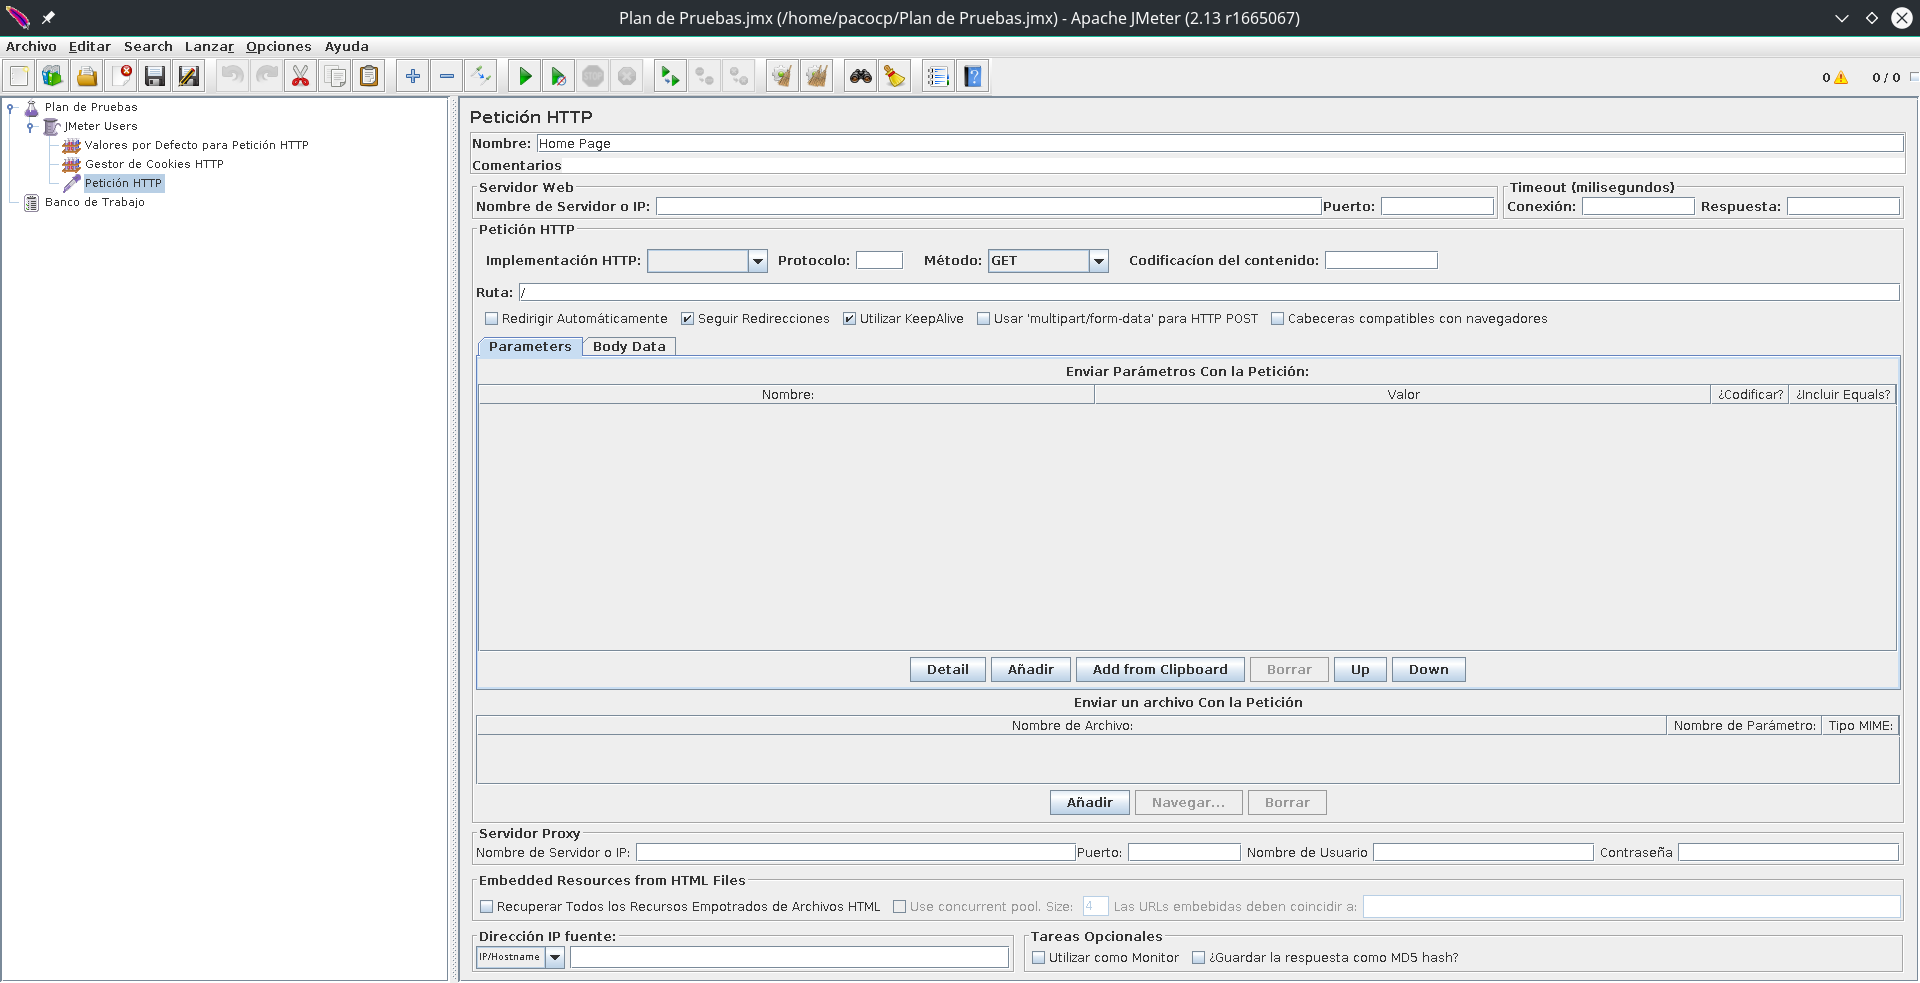
\includegraphics[scale=0.35]{figuras/figura19.png}  %el parámetro scale permite agrandar o achicar la imagen. En el nombre de archivo puede especificar directorios
	
	
	\caption{Añadiendo un muestreador de petición HTTP}
	\label{figura19}
\end{figure}

\begin{figure}[H] %con el [H] le obligamos a situar aquí la figura
	\centering
	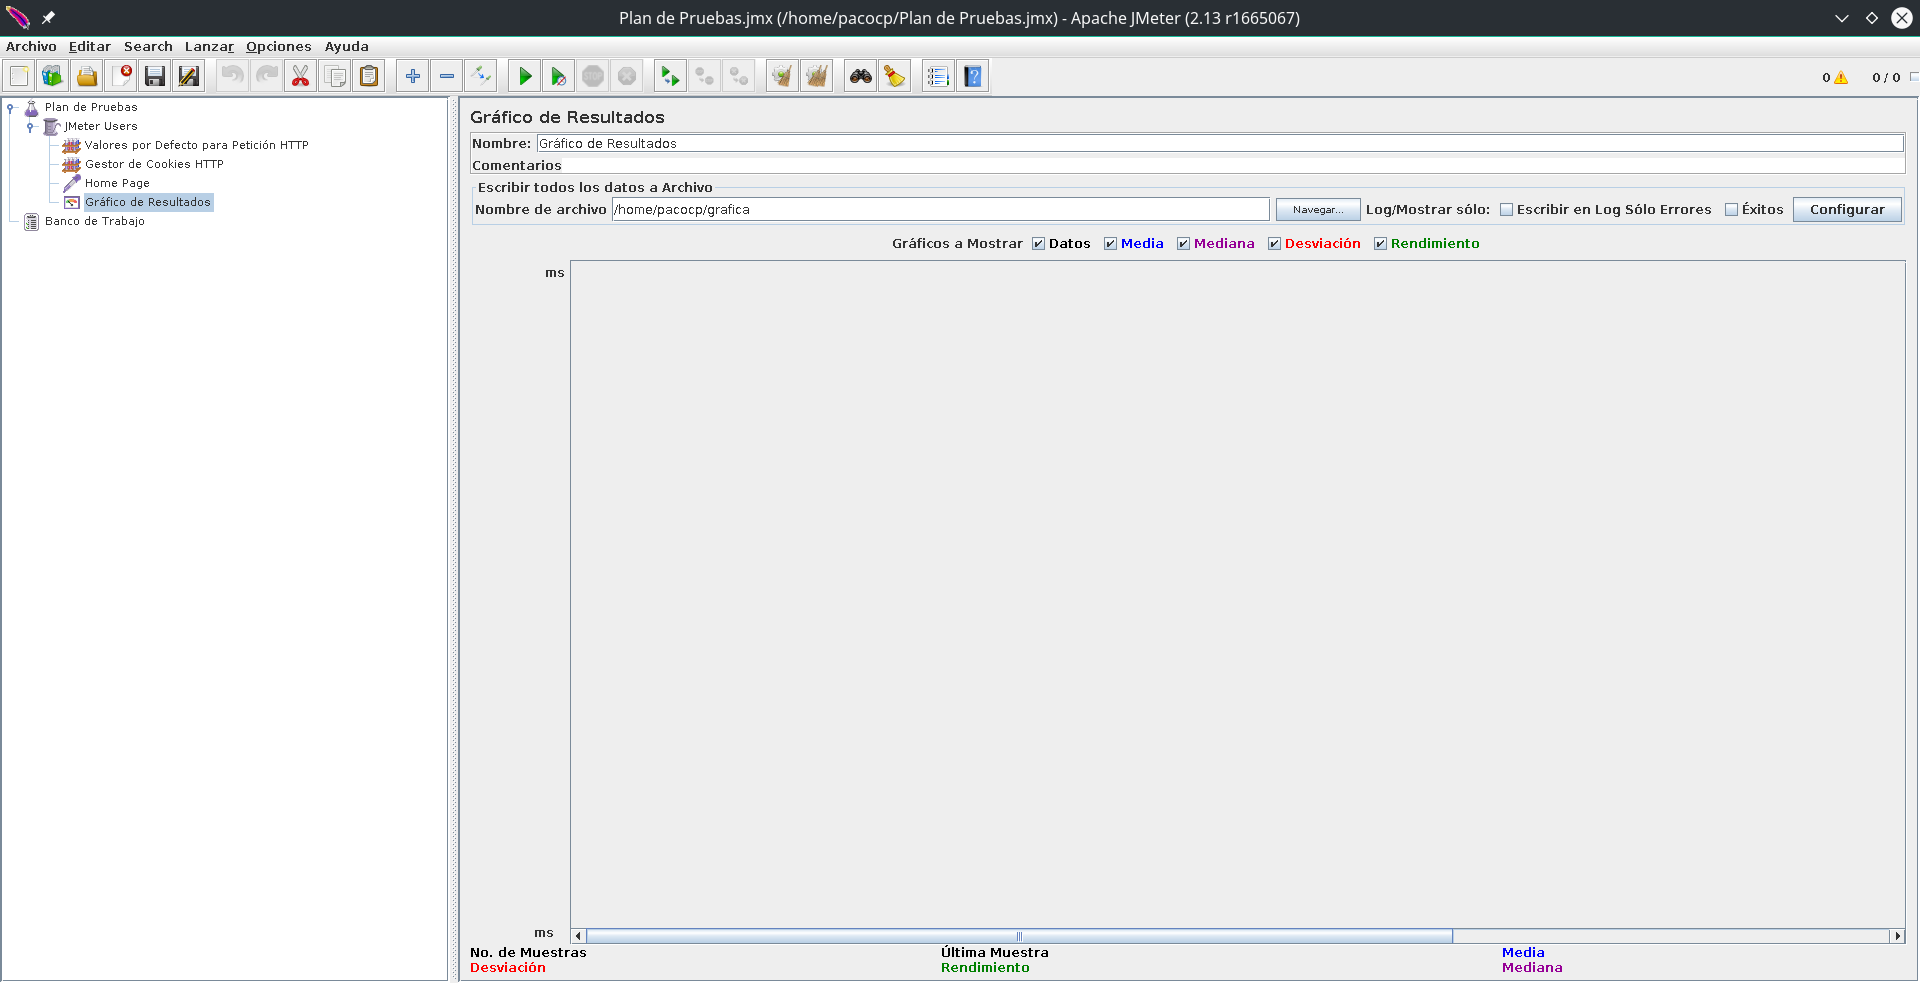
\includegraphics[scale=0.35]{figuras/figura20.png}  %el parámetro scale permite agrandar o achicar la imagen. En el nombre de archivo puede especificar directorios
	
	
	\caption{Configuramos un receptor con una gráfica de resultados}
	\label{figura20}
\end{figure}

\begin{figure}[H] %con el [H] le obligamos a situar aquí la figura
	\centering
	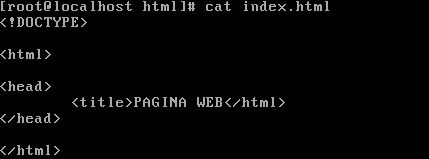
\includegraphics[scale=0.35]{figuras/figura23.png}  %el parámetro scale permite agrandar o achicar la imagen. En el nombre de archivo puede especificar directorios
	
	
	\caption{Página web simple HTML}
	\label{figura23}
\end{figure}

\begin{figure}[H] %con el [H] le obligamos a situar aquí la figura
	\centering
	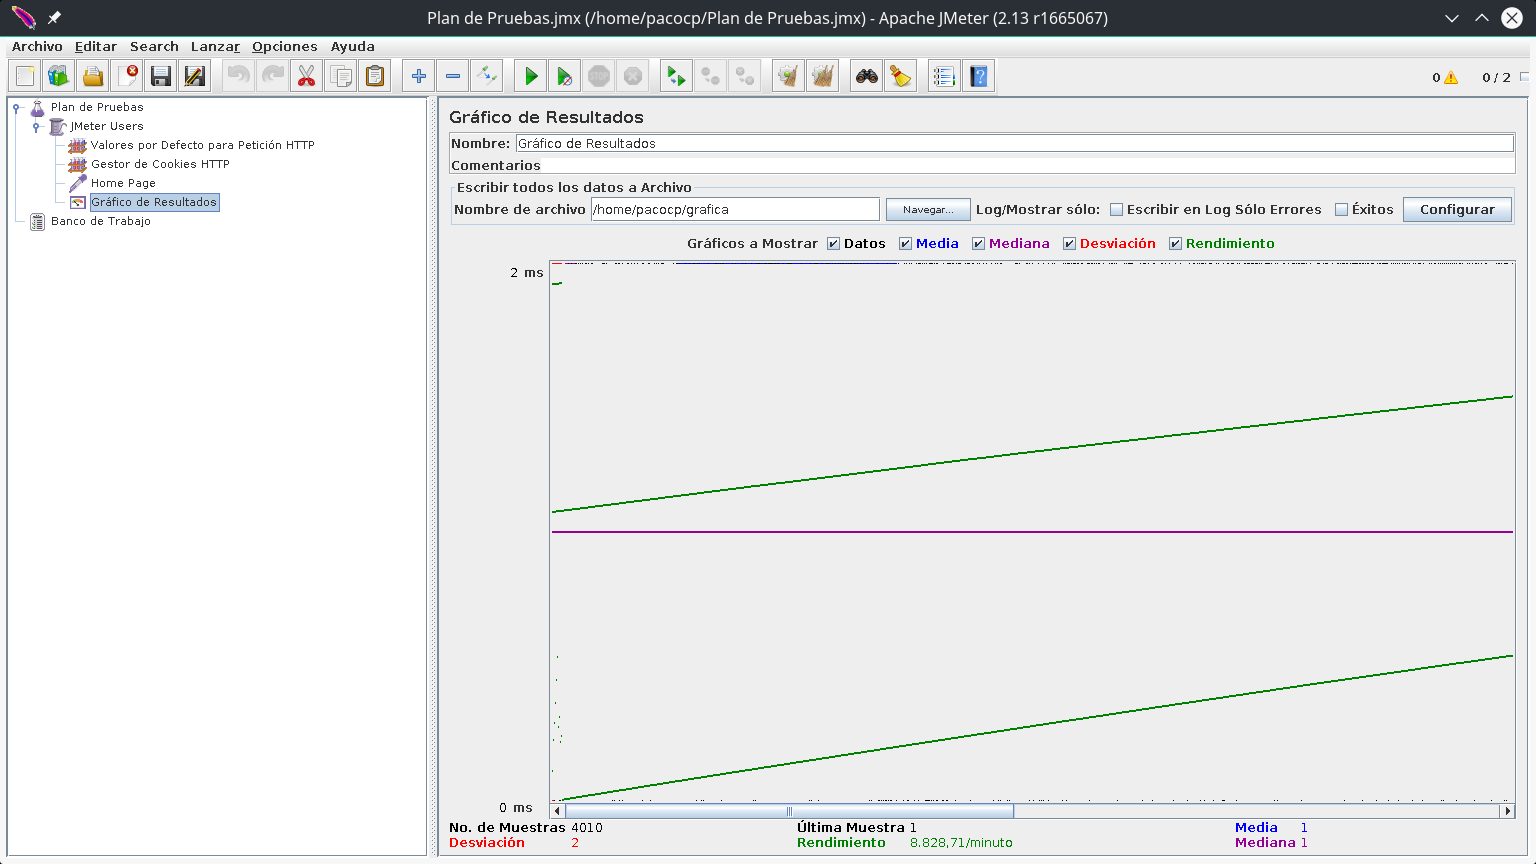
\includegraphics[scale=0.35]{figuras/figura24.png}  %el parámetro scale permite agrandar o achicar la imagen. En el nombre de archivo puede especificar directorios
	
	
	\caption{Resultado de ejecutar el test}
	\label{figura24}
\end{figure}

%%%%%%%%%%%%%%%%%%%%%%%%%%%%%%%%%%%%%%%%%%%%%%%%%%%%
% CUESTIÓN 4
%%%%%%%%%%%%%%%%%%%%%%%%%%%%%%%%%%%%%%%%%%%%%%%%%%%%

\section{Cuestión 5: Programe un benchmark usando el lenguaje que desee.}

A continuación voy a mostrar el código del benchmark, realizado en Python.\\
\begin{lstlisting}[language=python]

#!/usr/bin/env python
# -*- coding:utf-8 -*-

from sys import argv
import subprocess
import time
import tkinter as tk

print("*******************************************")
print("*                                         *")
print("*         BENCHMARK WEB LANGUAGES         *")
print("*                                         *")
print("*******************************************\n")

#subprocess.call(["TIMEFORMAT='%R'"]) #Formato solo en segundos y solo el real time

subprocess.call(['echo','>',"python-bubble.dat"])
subprocess.call(['echo','>',"perl-bubble.dat"])
subprocess.call(['echo','>',"php-bubble.dat"])
subprocess.call(['echo','>',"read.dat"])
subprocess.call(['echo','>',"write.dat"])


f = open('python-bubble.dat','w')
g = open('perl-bubble.dat','w')
h = open('php-bubble.dat','w')

print("*****************************************************\n")
print("Your system specs are: \n")
subprocess.call(['lscpu'])
print("*****************************************************\n")

print("We are going to execute the following scripts and measure the execution time.\n")

print("First of all, let's execute the BubbleSort algorithm in each language.\n")

medium_python = []
medium_php = []
medium_perl = []
media_python = 0
media_perl = 0
media_php = 0
index = 0
orden = 1 #This value is going to be necessary to determinate the order of scripts execution

for i in range(1000, 10000,1000):
medium_python.append(0)
medium_perl.append(0)
medium_php.append(0)

for i in range(0,10,1):
orden = orden + 1
if(orden > 3):
orden = 1
index = 0
for i in range(1000, 10000, 1000):
#f.write(str(i)+" ")
#g.write(str(i)+" ")
#h.write(str(i)+" ")

if(orden == 1):
print("PYTHON\n")
start = time.time()
subprocess.call(['python','bubblesort.py',str(i)])
end = time.time()
medium_python[index] = medium_python[index] + (end - start)
#f.write(str(data)+"\n")

print("PHP\n")
start = time.time()
subprocess.call(['php','bubblesort.php',str(i)])
end = time.time()
medium_php[index] = medium_php[index] + (end - start)
#h.write(str(data)+"\n")

print("PERL\n")
start = time.time()
subprocess.call(['perl','bubblesort.pl',str(i)])
end = time.time()
medium_perl[index] = medium_perl[index] + (end - start)
#g.write(str(data)+"\n")
if(orden == 2):
print("PHP\n")
start = time.time()
subprocess.call(['php','bubblesort.php',str(i)])
end = time.time()
medium_php[index] = medium_php[index] + (end - start)
#h.write(str(data)+" ")

print("PERL\n")
start = time.time()
subprocess.call(['perl','bubblesort.pl',str(i)])
end = time.time()
medium_perl[index] = medium_perl[index] + (end - start)
#g.write(str(data)+"\n")

print("PYTHON\n")
start = time.time()
subprocess.call(['python','bubblesort.py',str(i)])
end = time.time()
medium_python[index] = medium_python[index] + (end - start)
#f.write(str(data)+" ")
if(orden == 3):
print("PERL\n")
start = time.time()
subprocess.call(['perl','bubblesort.pl',str(i)])
end = time.time()
medium_perl[index] = medium_perl[index] + (end - start)
#g.write(str(data)+"\n")

print("PHP\n")
start = time.time()
subprocess.call(['php','bubblesort.php',str(i)])
end = time.time()
medium_php[index] = medium_php[index] + (end - start)
#h.write(str(data)+" ")

print("PYTHON\n")
start = time.time()
subprocess.call(['python','bubblesort.py',str(i)])
end = time.time()
medium_python[index] = medium_python[index] + (end - start)
#f.write(str(data)+" ")

index = index + 1



index = 0
for i in range(1000, 10000,1000):
f.write(str(i)+" ")
g.write(str(i)+" ")
h.write(str(i)+" ")

f.write(str(medium_python[index]/10) + "\n")
g.write(str(medium_perl[index]/10) + "\n")
h.write(str(medium_php[index]/10) + "\n")

index = index + 1

f.close()
g.close()
h.close()

#####################################
print("Now let's creat the file for testing reading a file, the size of the file is 50MB\n")
subprocess.call(['dd','if=/dev/zero','of=testfile_50MB','bs=50485760','count=1'])


media_python2 = 0
media_php2 = 0
media_perl2 = 0
print("Now test reading a file. We are going to do two test in one. We are going to read from RAM and from HD\n")
#TEST LECTURA
orden = 1
for i in range(0,10,1):
if(orden == 1):
print("PYTHON\n")
start = time.time()
subprocess.call(['python','readfile.py','testfile_50MB'])
end = time.time()
media_python = media_python + (end - start)

#f.write(str(data)+"\n")

print("PHP\n")
start = time.time()
subprocess.call(['php','readfile.php','testfile_50MB'])
end = time.time()
media_php = media_php + (end - start)

#h.write(str(data)+"\n")

print("PERL\n")
start = time.time()
subprocess.call(['perl','readfile.pl','testfile_50MB'])
end = time.time()
media_perl = media_perl + (end - start)

#g.write(str(data)+"\n")
if(orden == 2):
print("PHP\n")
start = time.time()
subprocess.call(['php','readfile.php','testfile_50MB'])
end = time.time()
media_php = media_php + (end - start)

#h.write(str(data)+" ")

print("PERL\n")
start = time.time()
subprocess.call(['perl','readfile.pl','testfile_50MB'])
end = time.time()
media_perl = media_perl + (end - start)

#g.write(str(data)+"\n")

print("PYTHON\n")
start = time.time()
subprocess.call(['python','readfile.py','testfile_50MB'])
end = time.time()
media_python = media_python + (end - start)

#f.write(str(data)+" ")
if(orden == 3):
print("PERL\n")
start = time.time()
subprocess.call(['perl','readfile.pl','testfile_50MB'])
end = time.time()
media_perl = media_perl + (end - start)
#g.write(str(data)+"\n")

print("PHP\n")
start = time.time()
subprocess.call(['php','readfile.php','testfile_50MB'])
end = time.time()
media_php = media_php + (end - start)

#h.write(str(data)+" ")

print("PYTHON\n")
start = time.time()
subprocess.call(['python','readfile.py','testfile_50MB'])
end = time.time()
media_python = media_python + (end - start)


orden = orden + 1
if(orden > 3):
orden = 1


f = open('read.dat','w')
f.write("0"+" "+"Python"+" "+str(media_python/10)+"\n")
f.write("1"+" "+"PHP"+" "+str(media_php/10)+"\n")
f.write("2"+" "+"Perl"+" "+str(media_perl/10)+"\n")
f.close()
#########################################
media_php = 0
media_python = 0
media_perl = 0
media_python2 = 0
media_php2 = 0
media_perl2 = 0
print("To sum up, we are going to test writing a file\n")
#TEST ESCRITURA
orden = 1
for i in range(0,10,1):
if(orden == 1):
print("PYTHON\n")
start = time.time()
subprocess.call(['python','writefile.py','write-py.txt'])
end = time.time()
media_python = media_python + (end - start)

#f.write(str(data)+"\n")

print("PHP\n")
start = time.time()
subprocess.call(['php','writefile.php','write-php.txt'])
end = time.time()
media_php = media_php + (end - start)

#h.write(str(data)+"\n")

print("PERL\n")
start = time.time()
subprocess.call(['perl','writefile.pl','write-pl.txt'])
end = time.time()
media_perl = media_perl + (end - start)

#g.write(str(data)+"\n")
if(orden == 2):
print("PHP\n")
start = time.time()
subprocess.call(['php','writefile.php','write-php.txt'])
end = time.time()
media_php = media_php + (end - start)
start = time.time()

#h.write(str(data)+" ")

print("PERL\n")
start = time.time()
subprocess.call(['perl','writefile.pl','write-pl.txt'])
end = time.time()
media_perl = media_perl + (end - start)
start = time.time()


print("PYTHON\n")
start = time.time()
subprocess.call(['python','writefile.py','write-py.txt'])
end = time.time()
media_python = media_python + (end - start)
start = time.time()

if(orden == 3):
print("PERL\n")
start = time.time()
subprocess.call(['perl','writefile.pl','write-pl.txt'])
end = time.time()
media_perl = media_perl + (end - start)
start = time.time()


print("PHP\n")
start = time.time()
subprocess.call(['php','writefile.php','write-php.txt'])
end = time.time()
media_php = media_php + (end - start)

#h.write(str(data)+" ")

print("PYTHON\n")
start = time.time()
subprocess.call(['python','writefile.py','write-py.txt'])
end = time.time()
media_python = media_python + (end - start)


orden = orden + 1
if(orden > 3):
orden = 1

f = open('write.dat','w')
f.write("0"+" "+"Python"+" "+str(media_python/10)+"\n")
f.write("1"+" "+"PHP"+" "+str(media_php/10)+"\n")
f.write("2"+" "+"Perl"+" "+str(media_perl/10)+"\n")
f.close()



######################################

print("Plotting the graphs\n")
subprocess.call(['gnuplot','gnuplot.gp'])

######################################

print("Deleting all the trash\n")

subprocess.call(['rm','write-py.txt','write-php.txt','write-pl.txt'
,'testfile_50MB'])

################################################

#This it's going to show the results in a pop-up window
print("Showing results\n")

root = tk.Tk()
root.title("Benchmark Web languages")
photo = tk.PhotoImage(file= r"writefile.gif")
photo2 = tk.PhotoImage(file = r"readfile.gif")
photo3 = tk.PhotoImage(file = r"bubblesortbenchmark.gif")
cv = tk.Canvas(root,width=2000, height=2000)
cv.pack(side='top', fill='both', expand='yes')
cv.create_text(950,100,font=("Purisa", 50),text = "BENCHMARK WEB LANGUAGES")
cv.create_image(5, 200, image=photo, anchor='nw')
cv.create_image(645, 200, image=photo2, anchor='nw')
cv.create_image(1280, 200, image=photo3, anchor='nw')
root.mainloop()


\end{lstlisting}

\subsection{Objetivo del benchmark}
El objetivo del benchmark es comparar la velocidad de ejecución de tres lenguajes web, en este caso Python, Perl y PHP, en tres tareas distintas. Estas tareas son, el algoritmo de ordenación Bubble Sort más la creación de un vector con elementos aleatorios para la prueba de mismo, la lectura de un archivo de 50MB y la escritura de un archivo de 6.6 MB . Con estos datos se representarán las gráficas donde podremos observar cuál es el vencedor en cada caso. 
\subsection{Métricas}
Las métricas que utiliza el benchmark son segundos para la ejecución, en el caso del Bubble Sort también tenemos el tamaño de los datos, que es simplemente el tamaño del vector que están ordenando. Para la medida de la lectura y escritura en archivos se toma el tiempo de ejecución y se mide en segundos. Y el tamaño de los archivos está indicado en la subsección anterior.\\ 
Se realizan 10 mediciones en todos los casos, y se saca la media de la suma de todas esas mediciones. En el caso del algoritmo de ordenación Bubble Sort más la creación de un vector con elementos aleatorios se realiza con vectores de números de entre 1000 a 9000 números.
\subsection{Instrucciones para su uso}
Las instrucciones son simples.Descomprimes el paquete que contiene todos los recursos, y ejecutas el comando \textbf{python benchmark.py} y ya se realiza todo automáticamente. Es decir, la realización del benchmark, le recolección de los datos, la creación de las gráficas y el posterior visonado de las mismas.\\
Para poder usarlo es necesario tener unos prerrequisitos: 
\begin{enumerate}
	\item Tener instalado Python 3.x, si utilizas Python 2.x será necesario que adaptes el código.
	\item Tener instalado el intérprete de PHP.
	\item Tener instalado el intérprete de Perl.
	\item Tener instalado gnuplot.
	\item Tener instalada la librería tkinder de Python, que se utilizará para mostrar los resultados.Se puede obtener siguiendo las siguientes instrucciones \cite{tk}. Si te encuentras en una distro basada en ArchLinux se encuentran en los repositorios extra con el nombre tk.
\end{enumerate}
\subsection{Ejemplo de uso analizando los resultados}
Ejecutamos el comando \textbf{python benchmark.py} y el programa nos va diciendo lo que va a ir realizando. Nos muestra las especificaciones de nuestra máquina como podemos observar en la Figura \ref{figura31}.\\
En todo el benchmark hay que tener en cuenta que a Python se le hace un favor ya que el script del benchmark está escrito en Python, por lo que el intérprete ya está cargado cuando se llama de nuevo para medir el tiempo que tarda en realizar las diferentes tareas.\\
Primero se va a realizar el algoritmo Bubble Sort más la creación de un vector de números aleatorios, cambiando en cada iteración el que ejecuta primero, ya que ese se lleva más carga.\\
A continuación, se realizan las mediciones para la lectura de disco, y por último la escritura en disco, siguiendo las mismas directrices que para las primeras mediciones.\\
Los datos nos los escribe en archivos .dat para luego poder dibujar las gráficas con gnuplot. Podemos observar como quedan en la Figura \ref{figura26} para la lectura de disco, en la Figura \ref{figura27} para la escritura en disco, en la Figura \ref{figura28} para el algoritmo Bubble Sort más la creación de un vector de números aleatorios en Python, en la Figura \ref{figura29} para el algoritmo Bubble Sort más la creación de un vector de números aleatorios en PHP, y por último en la Figura \ref{figura29} para el algoritmo Bubble Sort más la creación de un vector de números aleatorios en Perl.\\
Crea las gráficas con el script de gnuplot de nombre \textbf{gnuplot.gp}, elimina los archivos basura que se han creado y nos muestra el resultado como se puede observar en la Figura \ref{figura25}.\\

A la vista de los resultados podemos ver que Perl y PHP son los ganadores en las distintas pruebas. En el algoritmo Bubble Sort más la creación de un vector de números aleatorios gana Perl por bastante, y también gana en la escritura en disco. Mientras que PHP gana en la lectura en disco. Python siempre queda en segundo lugar en las tres pruebas realizadas. Desde el punto de vista personal y valorando al diferencia en los resultados, Python sería la mejor opción debido a varios factores:
\begin{itemize}
	\item Su curva de aprendizaje es mucho menor que la de Perl. Aunque Perl sea más rápido en esos dos casos, la cantidad de horas que he pasado buscando documentación no vale la pena.
	\item Relacionado con lo anterior, la cantidad de información y la calidad de la documentación de Python es extraordinaria.
	\item Además, la diferencia entre los resultados no es tan grande.
\end{itemize}

Pero esto siempre depende de para lo que vayamos a usar nuestro servidor. Y por supuesto, nuestra opinión personal.

\begin{figure}[H] %con el [H] le obligamos a situar aquí la figura
	\centering
	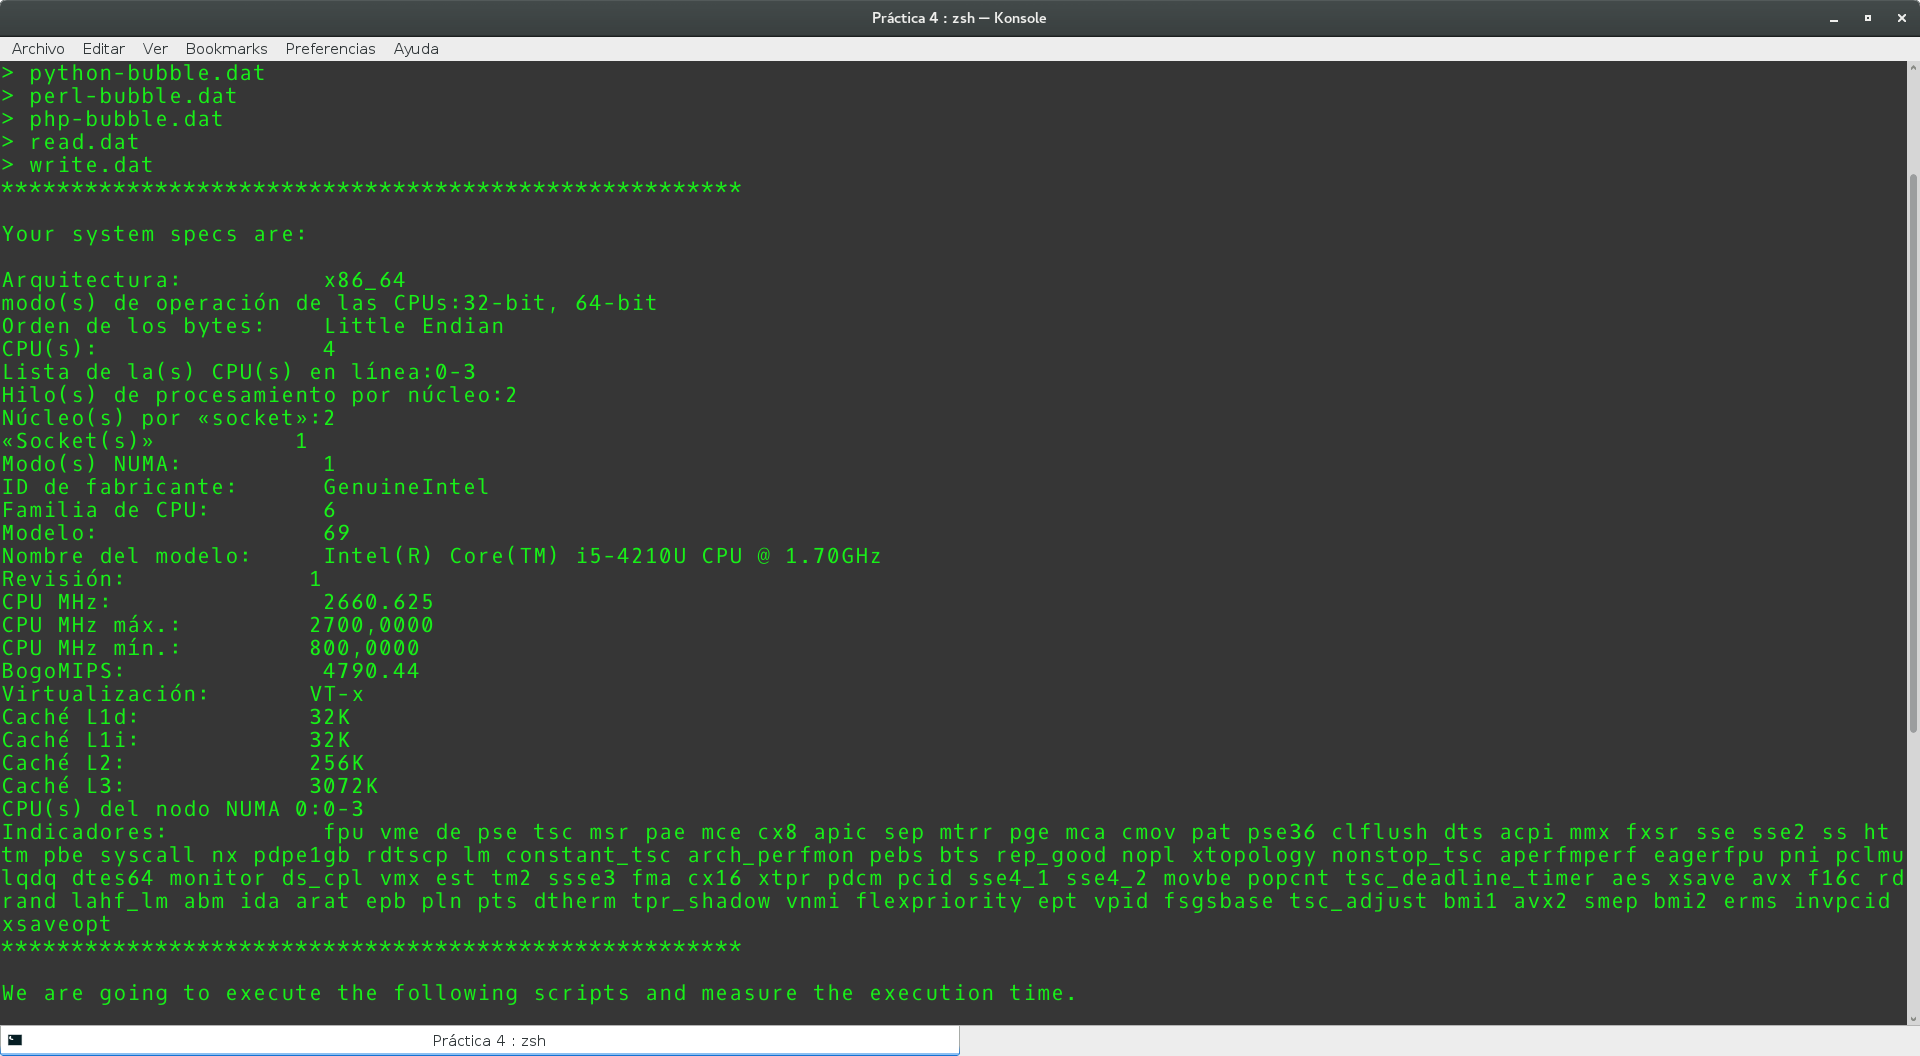
\includegraphics[scale=0.25]{figuras/figura31.png}  %el parámetro scale permite agrandar o achicar la imagen. En el nombre de archivo puede especificar directorios
	
	
	\caption{Especificaciones de la máquina}
	\label{figura31}
\end{figure}

\begin{figure}[H] %con el [H] le obligamos a situar aquí la figura
	\centering
	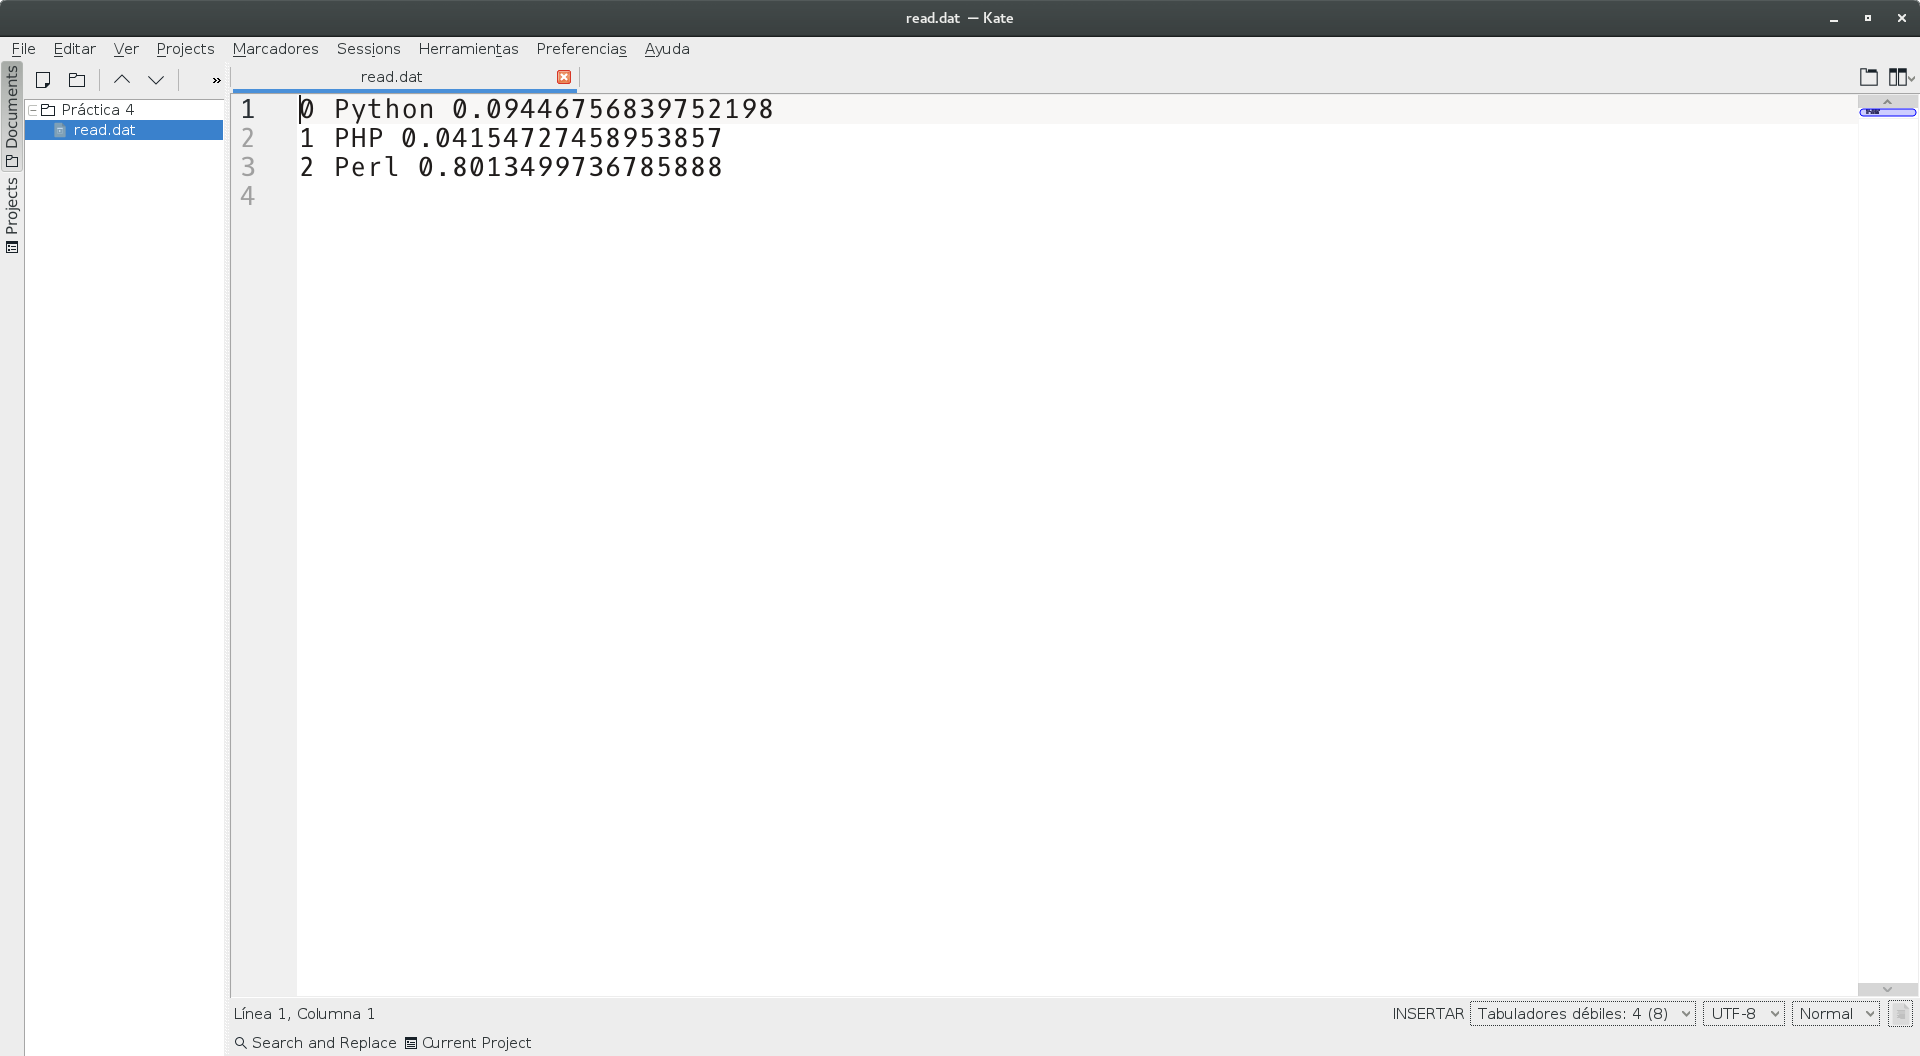
\includegraphics[scale=0.25]{figuras/figura26.png}  %el parámetro scale permite agrandar o achicar la imagen. En el nombre de archivo puede especificar directorios
	
	
	\caption{Lectura de disco}
	\label{figura26}
\end{figure}

\begin{figure}[H] %con el [H] le obligamos a situar aquí la figura
	\centering
	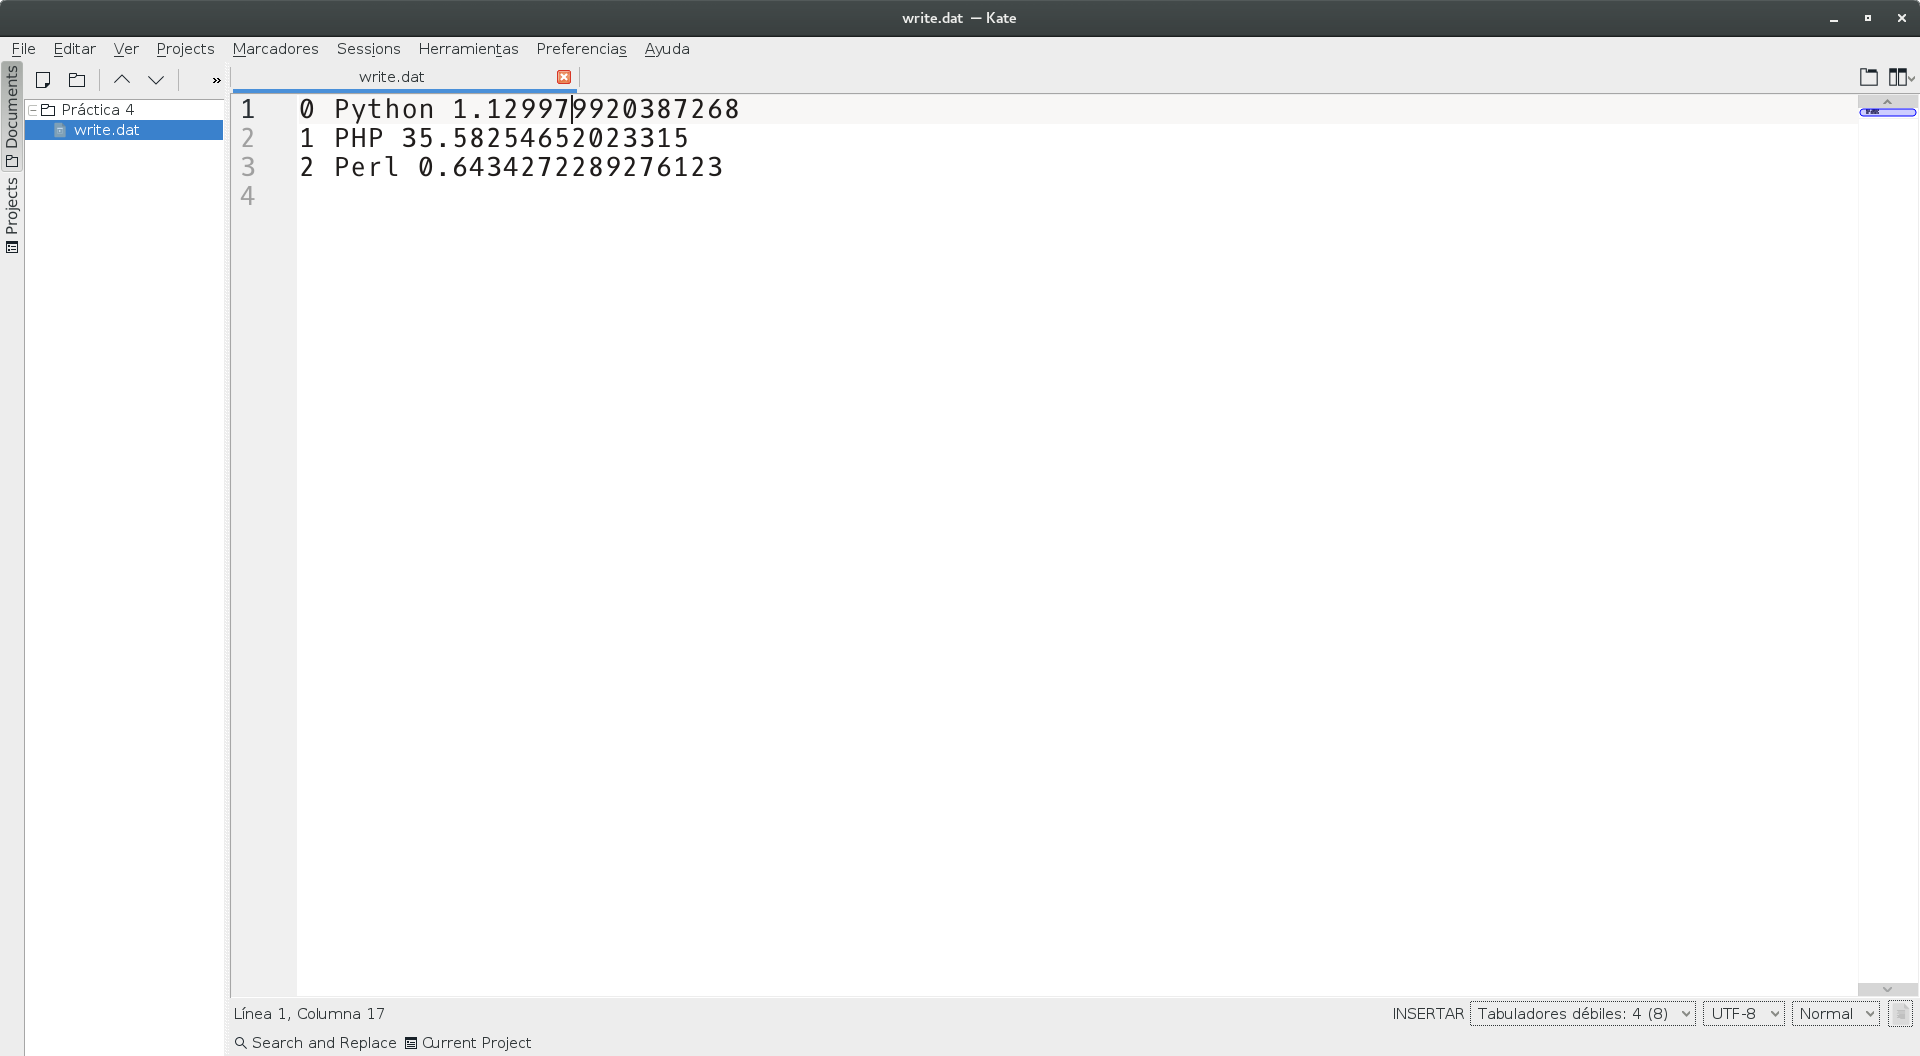
\includegraphics[scale=0.25]{figuras/figura27.png}  %el parámetro scale permite agrandar o achicar la imagen. En el nombre de archivo puede especificar directorios
	
	
	\caption{Escritura en disco}
	\label{figura27}
\end{figure}

\begin{figure}[H] %con el [H] le obligamos a situar aquí la figura
	\centering
	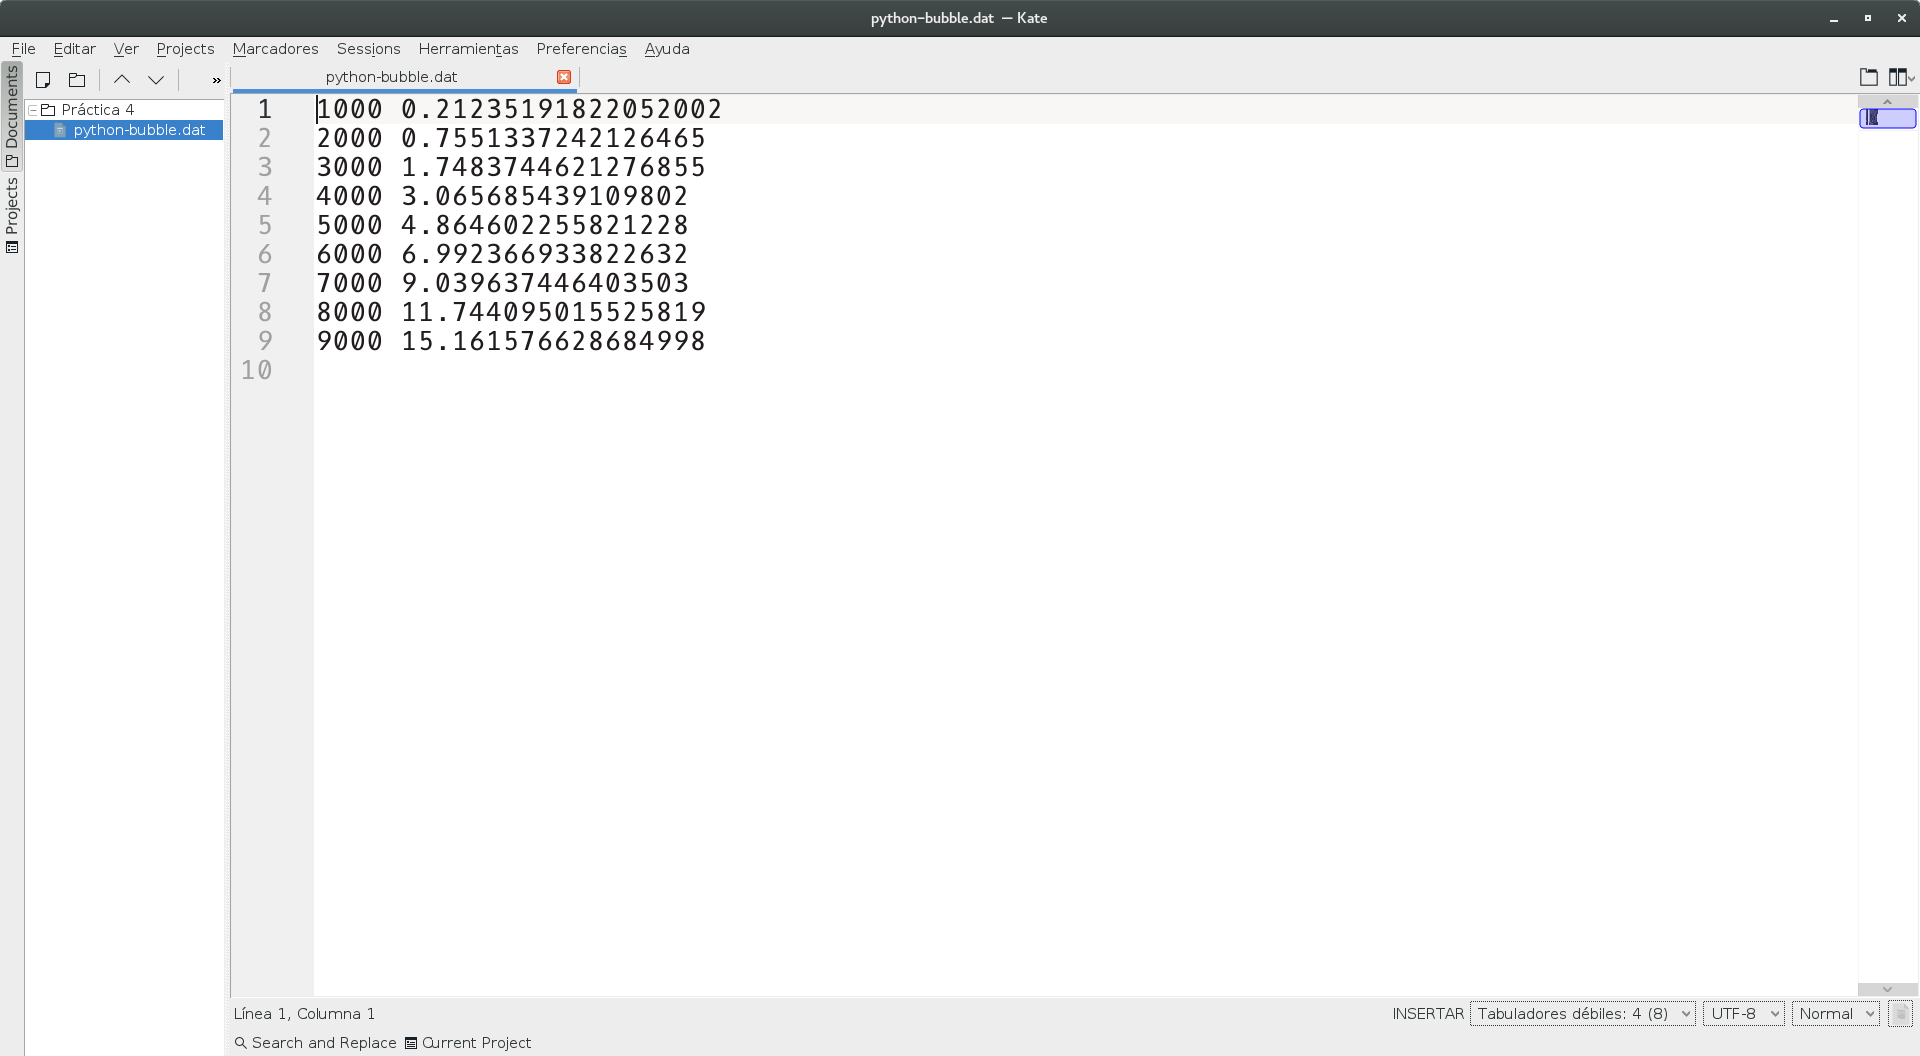
\includegraphics[scale=0.25]{figuras/figura28.png}  %el parámetro scale permite agrandar o achicar la imagen. En el nombre de archivo puede especificar directorios
	
	
	\caption{Algoritmo Bubble Sort más la creación de un vector de números aleatorios en Python}
	\label{figura28}
\end{figure}

\begin{figure}[H] %con el [H] le obligamos a situar aquí la figura
	\centering
	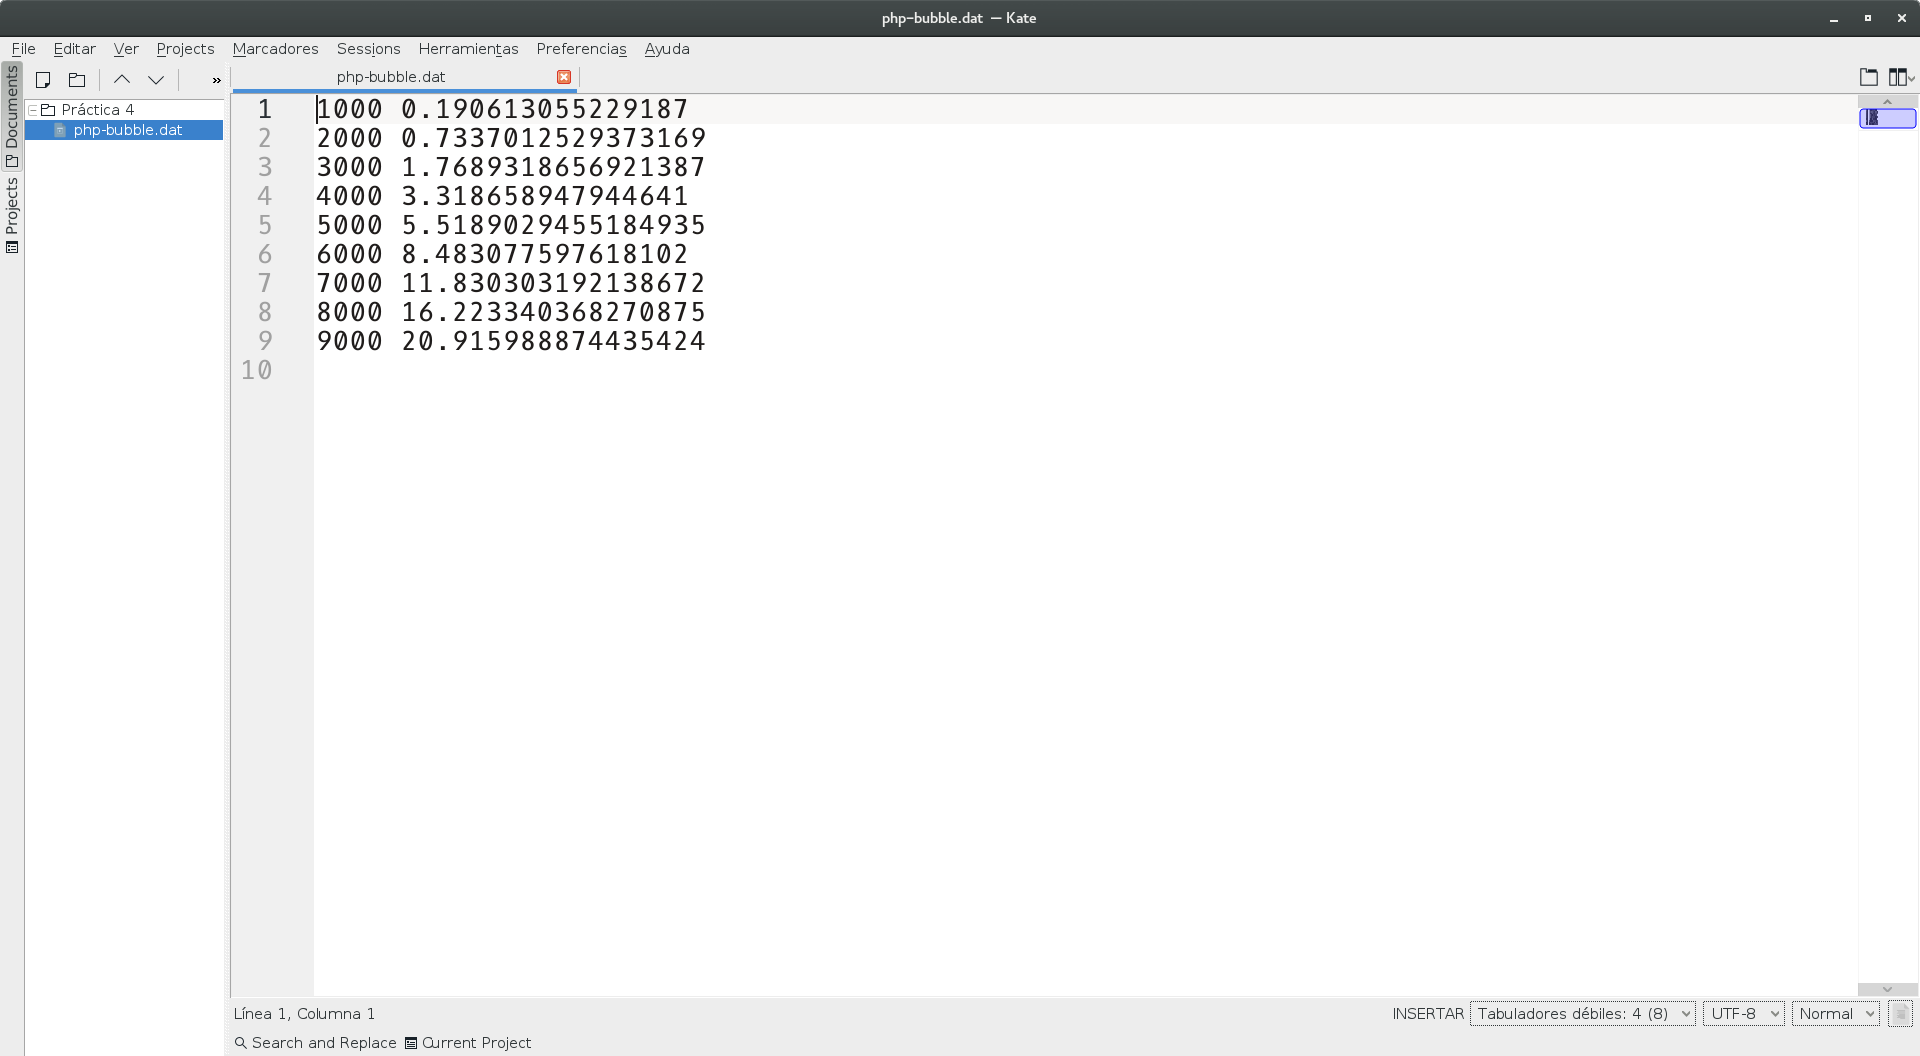
\includegraphics[scale=0.25]{figuras/figura29.png}  %el parámetro scale permite agrandar o achicar la imagen. En el nombre de archivo puede especificar directorios
	
	
	\caption{Algoritmo Bubble Sort más la creación de un vector de números aleatorios en PHP}
	\label{figura29}
\end{figure}

\begin{figure}[H] %con el [H] le obligamos a situar aquí la figura
	\centering
	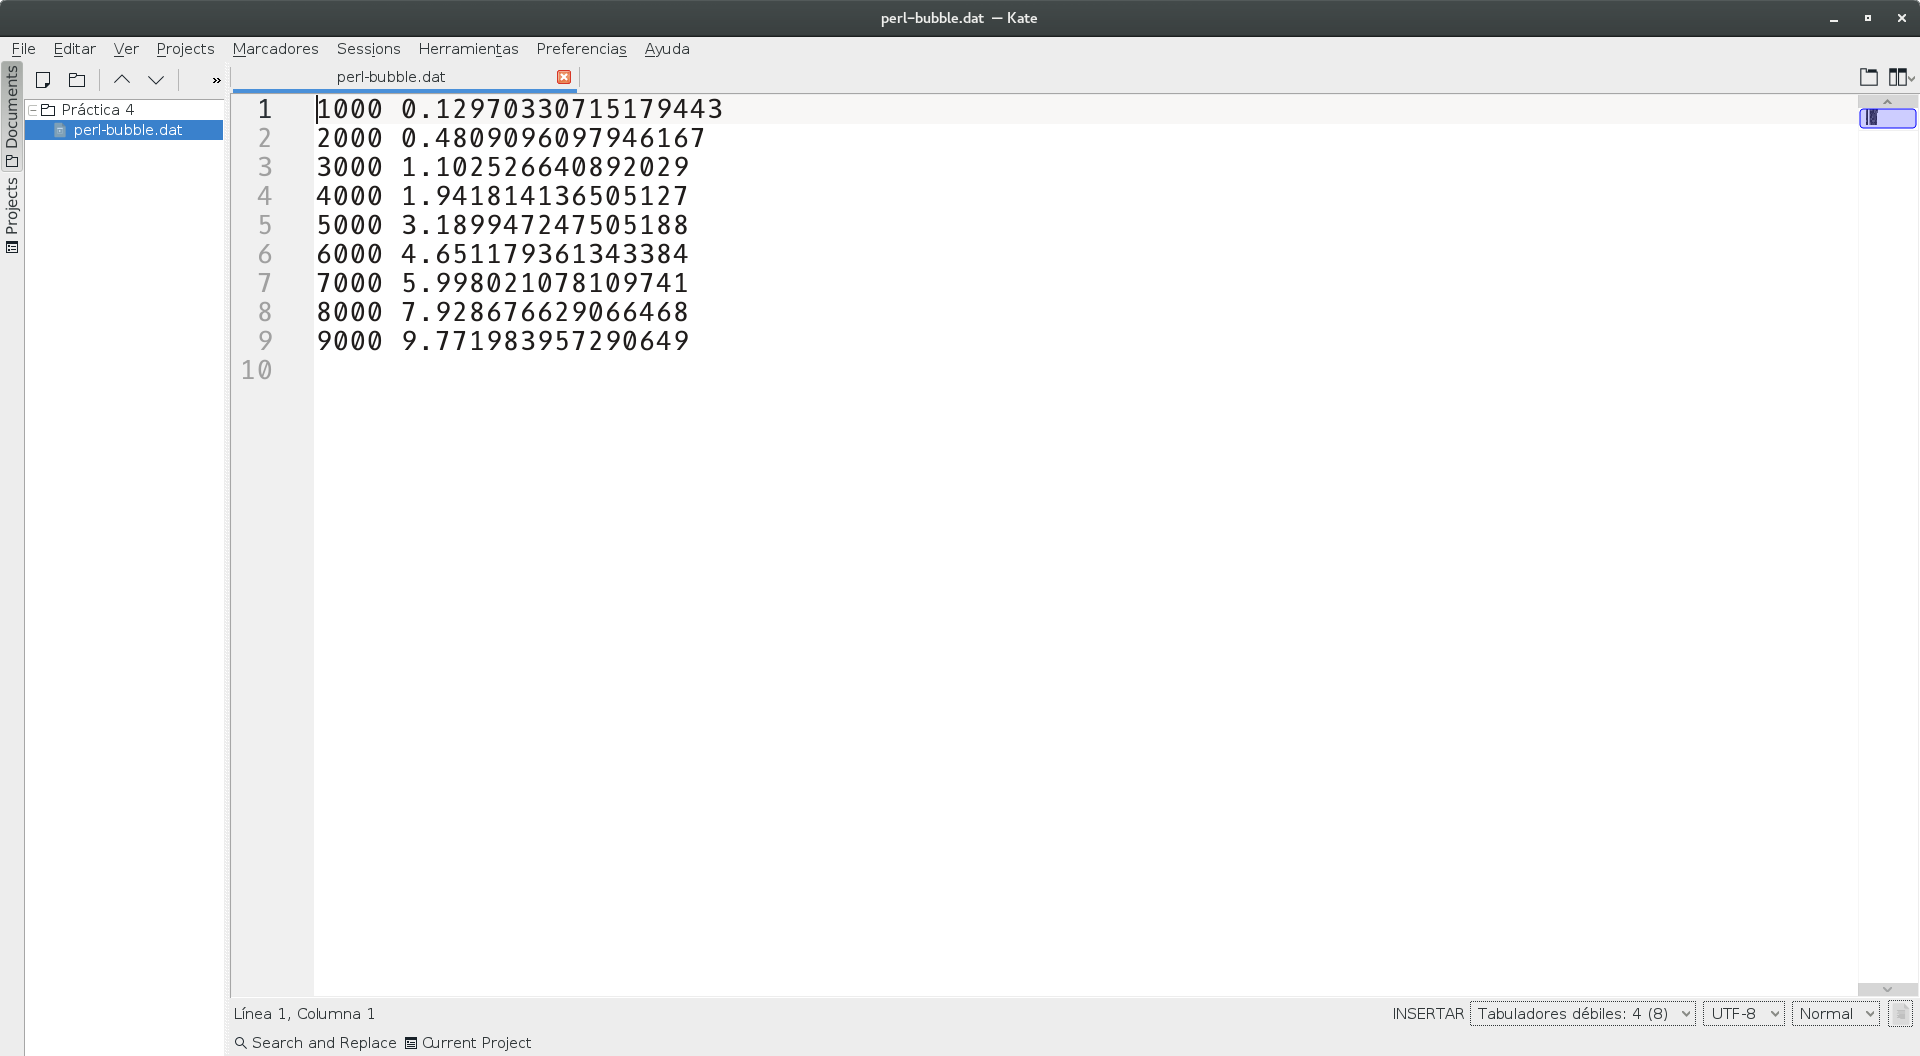
\includegraphics[scale=0.25]{figuras/figura30.png}  %el parámetro scale permite agrandar o achicar la imagen. En el nombre de archivo puede especificar directorios
	
	
	\caption{Algoritmo Bubble Sort más la creación de un vector de números aleatorios en Perl}
	\label{figura30}
\end{figure}

\begin{figure}[H] %con el [H] le obligamos a situar aquí la figura
	\centering
	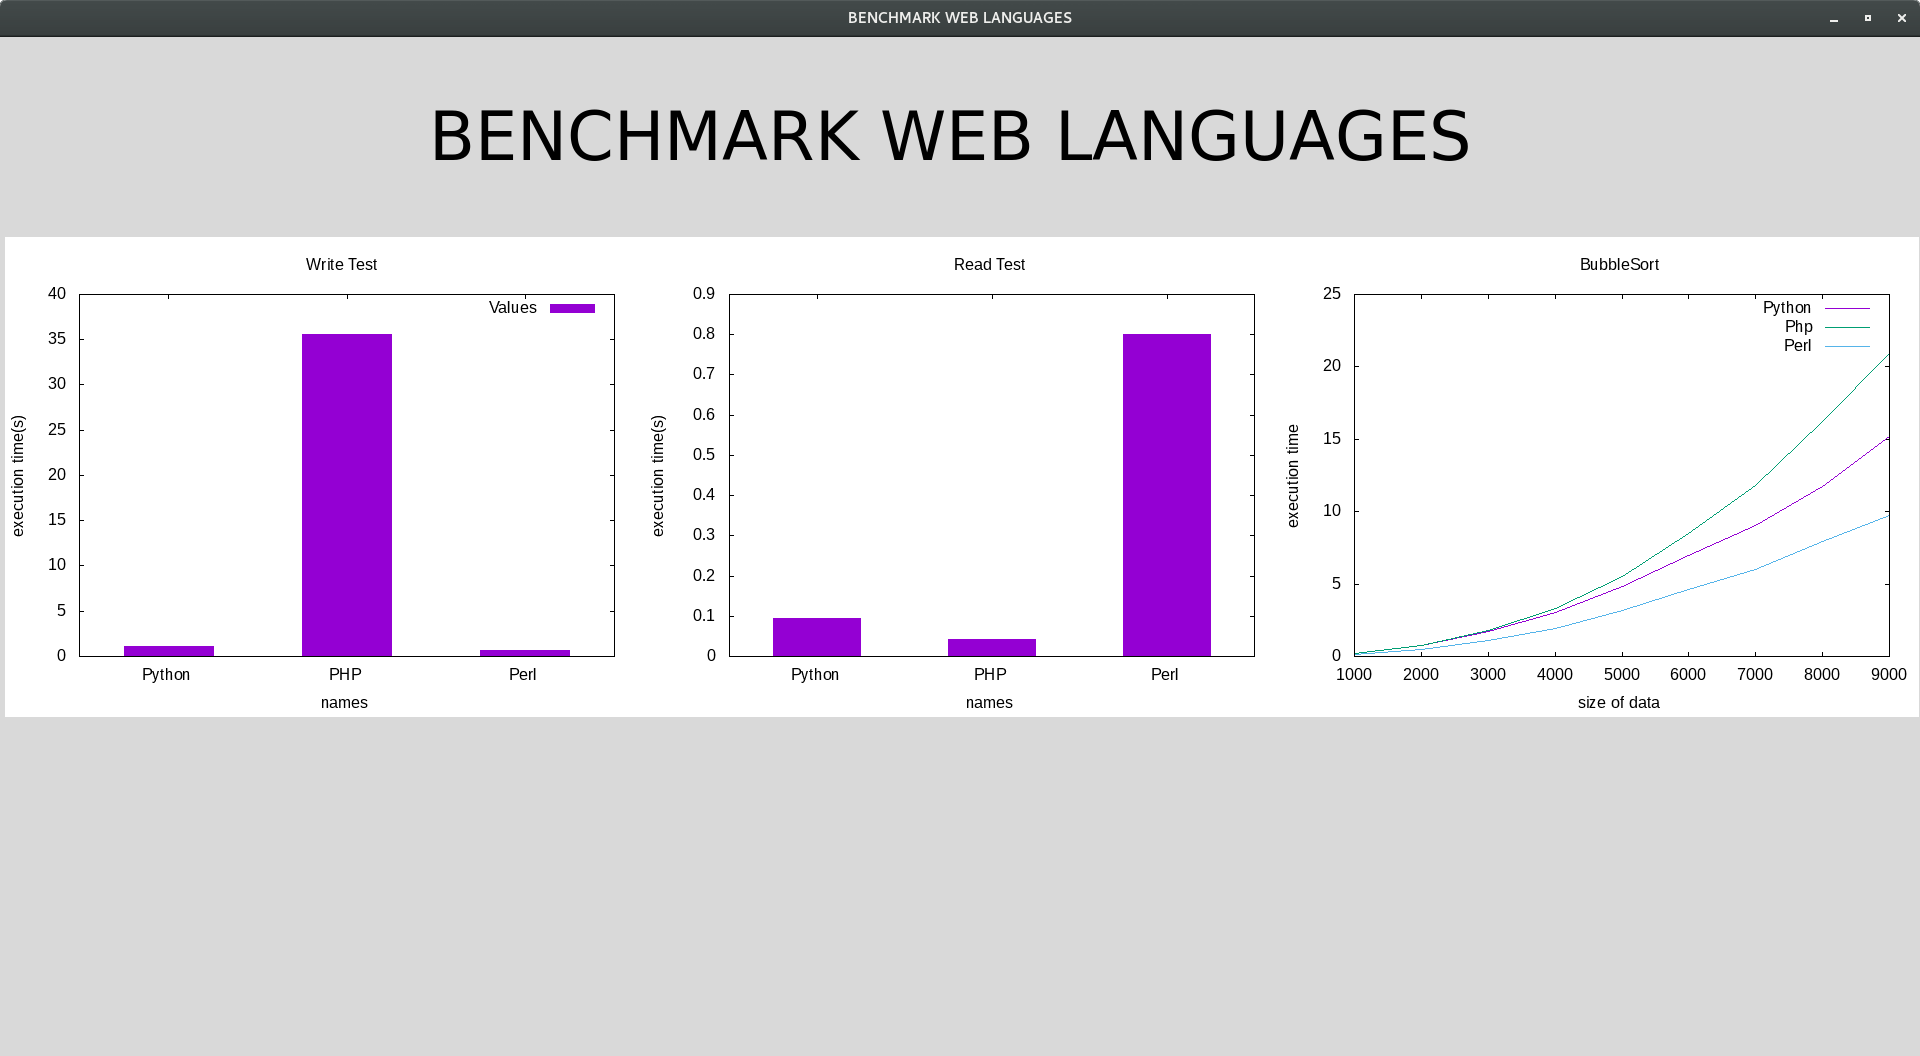
\includegraphics[scale=0.25]{figuras/figura25.png}  %el parámetro scale permite agrandar o achicar la imagen. En el nombre de archivo puede especificar directorios
	
	
	\caption{Resultados del Benchmark}
	\label{figura25}
\end{figure}
\newpage
\bibliography{citas} %archivo citas.bib que contiene las entradas 
\bibliographystyle{ieeetr} % hay varias formas de citar
\end{document}